 \chapter{HArBoUR: Heterogeneous Architecture Benchmarking on Unified Resources}\label{Harbour}

%Harbench - Heterogeneous Architecture Benchmarking
%HArIBoUR - Heterogeneous Architecture Imaging Benchmarking on Unified Resources
%HArbour-IP

This chapter presents a description of \textit{HArBoUR}, a heterogeneous imaging framework used for guidance and implementation of various image processing algorithms presented in later chapters. In addition, the chapter contains benchmarks and evaluations of micro/macro image processing algorithms commonly found in imaging pipelines of vision systems. The algorithm suitability on a specific accelerator is determined from the analysis of the results.

\label{chap:HFrwk}
\section{Introduction}
The advances in multi-core processors and accelerators have enabled real-time embedded imaging algorithms to become ubiquitous within many vision application areas such as advanced driver assist systems (ADAS) \cite{GeiFraCha18}, surveillance\cite{FabBerFra07} and satellites\cite{BruBruHin15}. The growing demand for image processing algorithms on systems with resource and energy constraints requires architectures that perform tasks efficiently. These hardware accelerators come with various architectures ranging from CPUs, GPUs, and FPGAs. Traditionally, embedded imaging designs often involve implementing image processing algorithms on homogeneous architectures, which come with hardware limitations. However, recent developments introduce heterogeneous architectures that combine multiple specialised accelerators on a singular interconnected chip\cite{Xilinx}. These novel architectures provide optimum design opportunities for embedded imaging development. However, current developments in targeting heterogeneous platforms are still primitive and require careful consideration of various development languages, tool-sets and performance profiles to fulfil energy and runtime constraints of applications. Furthermore, certain accelerators have pre-written optimised vision libraries, \eg OpenCV/CUDA (for CPU/ GPU) and xfOpenCV (for FPGAs). However, the design and development of image processing algorithms in a heterogeneous environment is still an arduous task. It requires in-depth knowledge of multiple hardware accelerators, and each differing in performance due to their underlying architectures. Additionally, FPGA designs require knowledge of hardware descriptor languages (HDLs), which have higher learning difficulty despite the existence of recent high-level synthesis tools or domain-specific languages that abstract away from the underlying hardware. This is due to a lack of understanding and the existence of benchmarks for image processing algorithms on different hardware. Therefore, partitioning complex image processing algorithms onto each accelerator remains a difficult task for application designers.

%The architecture enables tasks to be executed on a particular processor efficiently. 

%This is due to a lack of understanding and the existence of benchmarks for image processing algorithms on different hardware.  

%Heterogeneous architecture designs can be composed of multi-core Central Processing Units (CPU), Graphics Processing Unit (GPU), Field-Programmable Gate Arrays (FPGA) or any other additional accelerators or co-processors.

%CPUs comprise multiple complex ALU units that enable SIMD (Single Instruction Multiple Data) instructions. GPUs contain thousands of simple cores paired with high bandwidth memory that can implement a high degree of parallel processing on large data streams. An FPGA contains a re-programmable matrix of interconnected configurable logic blocks (CLBs) to allow signals to be routed and enable users to design custom logic and functions to only consume the power needed to execute the operation, improving energy efficiency. 

Benchmarking has played an integral part within the computing domain for decades. Since the beginning of computing systems, there has been a persistent need to evaluate and compare the performance of hardware components. Initially, with the early day mainframe computers to the modern era of microprocessors, GPUs, and custom ASICs, benchmarking has provided a standardised measure to gauge the efficiency, speed, and capabilities of hardware devices. Over the years, benchmarking tools and suites have played a pivotal role in driving technological advancements, guiding design decisions, and ensuring that hardware meets the ever-evolving demands of software applications. 

To address the emerging demand for high performance vision hardware, there is a need for a suitable benchmarking framework that dissects the imaging/vision algorithms in a disciplined way and benchmarks their performances (both energy and execution time) on all available target hardware (\eg CPU, GPU and FPGA). To address such a gap, this chapter proposes a new framework providing a systematic way of implementing imaging designs on specialised platforms and perform benchmarks on representative vision algorithms while assessing execution time, memory latency and energy consumption. System designers will use the proposed framework to identify appropriate hardware for the target application and unlock the potential of a true heterogeneous system. The main contributions of this chapter are:
\begin{itemize}
\item We propose a framework that studies features of image processing algorithms to identify characteristics. These characteristics help partition complex algorithms into the most optimal target accelerators within heterogeneous architectures.

\item The approach adopts a systemic and multi-layer strategy that offers trade-offs between runtime, energy and accuracy within the imaging sub-domains \eg \textit{CNNs} and \textit{feature extraction.} Specifically, \textit{HArBoUR} enables support in constructing end to end vision systems while providing expected results and guidance.

\item Domain knowledge-guided hardware evaluation of computational tasks allows imaging algorithms to be mapped onto hardware platforms more efficiently than a heuristic based approach.

\item We benchmark representative image processing algorithms on various hardware platforms and measure their \emph{energy consumption} and \emph{execution time} performance. The results are evaluated to gain insight into why certain processing accelerators perform better or worse based on the characteristics of the imaging algorithm.
  
%  \item  The results are evaluated to gain insight into why certain processing accelerators perform better or worse based on the characteristics of the image processing algorithm.
\end{itemize}





\section{Benchmarking Framework for Image Processing on Hardware}\label{sec:framework}
%--------------------------------------------------------
\begin{figure}[tb]
\centering
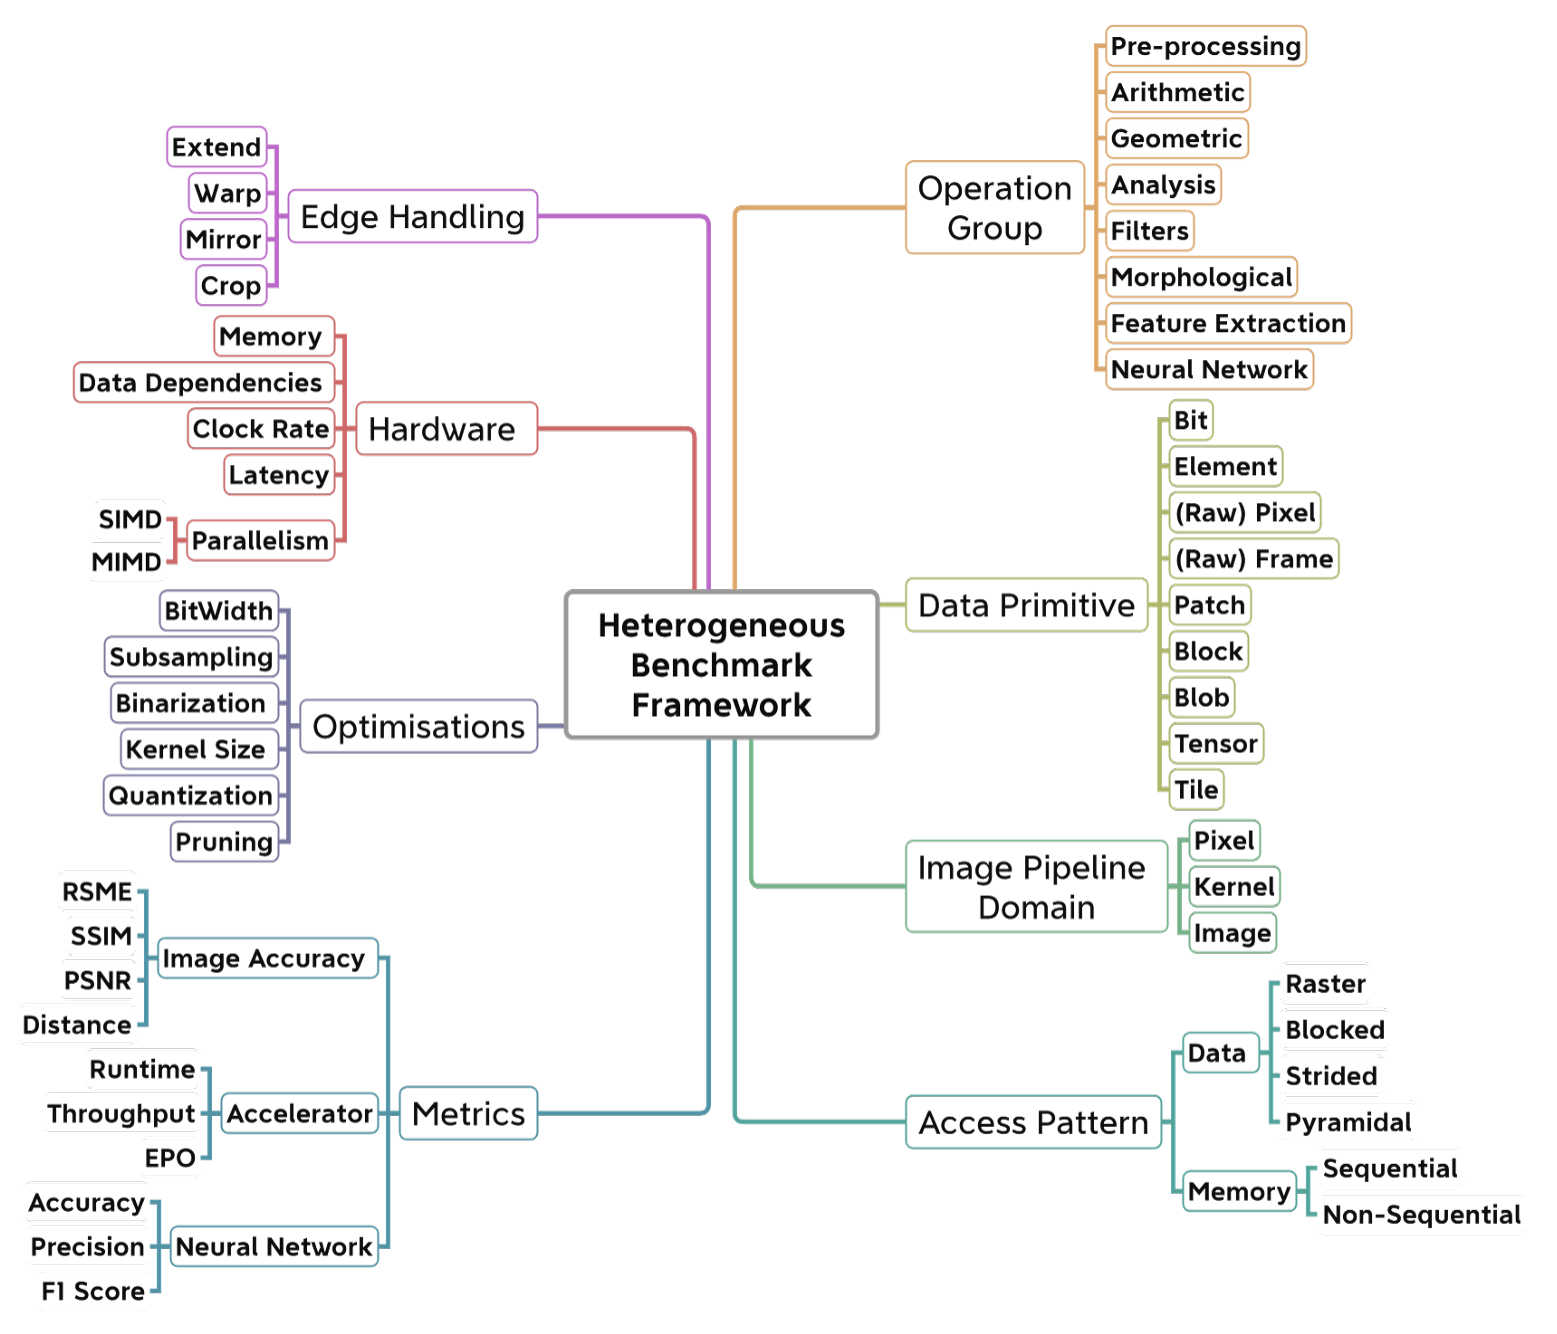
\includegraphics[width=\linewidth]{Images/Heterogeneous Benchmark Framework.png}
\caption[Benchmarking Framework]{Benchmarking Framework for Image Processing Algorithms, Highlighting Key Metrics and Properties}
\label{fig:AlgoChar}
\end{figure}
%--------------------------------------------------------
For efficient implementation on heterogeneous platforms, the algorithm design will require partitioning any image processing algorithm according to its suitability for individual components in the pipeline on the target hardware. Therefore, a standard framework is proposed containing a pool of image processing algorithms and their characteristics in accordance with their hardware suitability. We selected a range of low, medium and high-level algorithms from the image processing hierarchical classification domain, providing wider coverage of commonly used operations performed within a vision application pipeline. 

Various algorithmic and hardware characteristics that would impact the performance are identified in the heterogeneous benchmark framework, shown in \Fig{AlgoChar}. The framework diagram offers a clear overview of the image processing landscape. It maps out the relationship between hardware properties, optimisations, algorithms, metrics and memory access patterns. This concise visual guide aids designers by offering insights into potential bottlenecks, suggesting areas for innovation, and guiding the fine-tuning of algorithms on heterogeneous platforms to achieve peak performance in imaging tasks.

\subsection{Processing Pipeline \& Operation Types:}
Image processing algorithms are organised into three primary domains: Pixel, Kernel, and Image. The \textit{Pixel domain} focuses on operations that manipulate or query individual pixel values. The \textit{Kernel domain} encompasses algorithms that utilise a small matrix (the kernel) to modify an image. Lastly, the \textit{Image domain} deals with operations that consider the image as a whole, where global features and patterns are essential for labelling.

\subsection{Operator Group }
This label specifies the name of the algorithm. Algorithms may perform a particular operation (\eg Image Arithmetic), but depending on the stage within the image computation pipeline, the data type of the pixel is defined differently and may contain additional values for calibration, such as a pedestal. It is necessary to be explicit when defining the algorithm within the framework. These image processing algorithms can further be categorised into groups (Operation Group) depending on the type of operation it performs.

\paragraph{Image Arithmetic \& Pre-Processing:} 
Image arithmetic and pre-processing are foundational steps in image processing pipelines, preparing images for subsequent analysis. These algorithms predominantly execute primitive operations to transform an input format into a desired one. They typically operate on individual pixels using localised data, which minimises task dependencies. While algorithms like multiplication, accumulation, squaring, magnitude determination, and weighting are arithmetically simple, most architectures can compute them with ease. Given their low initialisation and latency requirements, architectures such as CPUs and FPGAs are particularly well-suited for these tasks.

\paragraph{Geometric Transformation \& Image Analysis:} 
Geometric transformations refer to operations that modify the spatial arrangement of pixels in an image. These transformations can be applied for various purposes, such as image registration, scaling, and augmentation. Typically, these algorithms involve convolution and interpolation operations, which can be linear or nonlinear. Additionally, the choice of interpolation method, whether nearest-neighbour, bilinear, or bicubic, can significantly impact both the quality of the transformed image and the computational complexity of the operation. Several operations are sequentially bound; forward mapping directly calculates new pixel locations but can leave gaps in the output. Its counterpart, backward mapping, determines source contributors for each output pixel and often requires interpolation, which can be sequential, especially with higher-order methods. Warping with a displacement map, which dictates pixel movement, can also be sequential if complex algorithms determine displacements. Resampling, essential post-mapping, can become sequential with intricate interpolation. Cumulative transformations, where multiple operations are applied in sequence, and error corrections post-transformation, further introduce sequential elements. For operations with inherent sequentiality, such as certain geometric transformations, traditional CPUs are often the most suitable due to their optimised instruction sets for sequential tasks and complex branching. However, for tasks within geometric transformations that can be parallelised, GPUs, FPGAs, and TPUs can offer significant speedups

Image analysis algorithms label and understand various statistical data about a pixel. These algorithms have many irregular memory access patterns (mean, mode, min/max) and branching conditions that negatively impact the performance of processing accelerators. 


\paragraph{Image Filters \& Morphology:} Image filter algorithms modify particular spatial frequencies. The image is filtered either in the frequency or in the spatial domain. Image filters are divided into two categories: linear and non-linear. Linear image filters perform the convolution of an image using a pre-computed kernel for efficiency. The data-independent multiply and accumulate operations coupled with sequential data access of linear filters map well onto GPUs and FPGAs. Contrarily, non-linear filters have varied memory access patterns and have higher arithmetic intensity. Additionally, certain algorithms with branching makes it arduous to implement efficiently on a GPU and FPGA, which can exploit parallelism in these operations. Non-linear filters consist of operations where the output pixel value is determined based on some non-linear function of the input pixel values in its neighbourhood. Examples of algorithms include median, adaptive and bilateral filtering.

In morphological operations, an image is processed with a structuring element, which is a small binary or grayscale mask. The structuring element is moved over the entire image, and at each position, a computation is performed based on the values of the image pixels that overlap with the mask. Architectures with cache hierarchies, prevalent in modern CPUs and GPUs, can exploit this pattern for enhanced cache locality, especially when the structuring element's dimensions are compatible with cache sizes. In row-major order, horizontal traversal optimises memory access, while vertical traversal can introduce inefficiencies due to memory strides. Basic operations like dilation and erosion have regular patterns, but advanced morphological algorithms can cause irregular accesses. These irregularities, often from adaptive structuring or conditional operations, challenge GPU performance through warp divergence. Additionally, these algorithms may require repeated pixel reads, especially with overlapping structuring elements, and in-place operations risk read-write conflicts, which need careful management to prevent race conditions.


\paragraph{Feature Extraction:} Feature extraction algorithms, such as SIFT\cite{Low99}, SURF\cite{Her06}, and Oriented FAST and Rotated BRIEF (ORB)\cite{ORB}, are designed to identify and describe local features in an image. These features are often points or small image patches that are distinct and can be reliably and robustly detected in various scales of the same scene. The pixels extracted from an image are not stored adjacently in memory and require expensive computational reads from non-adjacent memory addresses that will impact the performance of all processing architectures. Algorithms such as \texttt{ORB} examine a circle of pixels around each candidate pixel. While each keypoint detection is independent and can be parallelised, the algorithm involves conditional checks, which can lead to divergent execution paths.

Regarding hardware suitability, CPUs have a layered hierarchy of caches, encompassing L1, L2, and L3. This architecture is good at offsetting the performance implications of non-sequential memory accesses. Therefore, algorithms with random access patterns, akin to the keypoint detection seen in SIFT or ORB, can leverage this hierarchical structure. Nevertheless, despite their proficiency, CPUs will lag in efficiency when confronted with parallel operations stages within the algorithms. GPUs and FPGAs, on the other hand, are geared towards the parallel processing tasks which are found during the convolution and  prefix sum stage. GPUs favour coalesced memory access, where adjacent threads reading consecutive memory locations achieve faster, more efficient data retrieval. Consequently, the random accesses, if frequent, can lead to performance dips due to the resulting uncoalesced memory transactions. However, TPUs are purpose-built for tensor operations, forming the basis of deep learning methodologies. Traditional feature extraction may not have direct advantages from TPUs unless they're integrated into a wider deep learning framework. 


%Some examples are: Addition, Logical (AND/OR/XOR/NOT), colour conversion, blending, channel combine.

\subsubsection{Data Primitive:}
This characteristic specifies the type of data unit or collection of pixels an algorithm operates on, encompassing attributes like type, size, and representation. Depending on the level of the pipeline, a pixel may refer to an individual or collection of bits of type \texttt{word},  \texttt{uint8} or \texttt{uint12}. The following are the various data primitives found within image processing:

\begin{itemize}
  \item \textbf{Bit:} Refers to individual bits in the binary representation of the image data, encompassing pixel values, metadata, file headers, and more, contingent on the file format.
  \item \textbf{Element:} Denotes a discrete scalar value, formed of bits, quantifying pixel attributes, like colour intensity or luminance.
  \item \textbf{Pixel:} Is a set of elements symbolising a point in an image, with formats such as RGB, YUV, or Bayer encoding.
  \item \textbf{Frame:} Is a structured pixel collection visualised in 2D or 3D, where the resolution indicates the total pixel count.
  \item \textbf{Patch:} Is a small frame subsection targeted by algorithms like blurring; a $3\times3$, $5\times5$ Kernel is a matrix sliding over the image, its values multiplied with corresponding patch pixels, and the results summed for a transformed image.
  \item \textbf{Block:} Pertains to a contiguous pixel group, typically of fixed dimensions like $8\times8$ or $16\times16$, serving as the atomic unit for algorithms, such as JPEG compression.
  \item \textbf{Blob:} Is an image region defined by properties like brightness, distinct from surrounding areas.
  \item \textbf{Tensor:} Is a multi-dimensional structure encapsulating complex data; a 2D tensor represents greyscale images, while a 3D tensor handles colour images, considering width, height, and colour channels. In deep learning, tensors provide a concise mathematical  representation of the problem.
  \item \textbf{Tile:} Is a unique image portion, often rectangular, acting as a processing or representation unit. Unlike overlapping patches, tiles traditionally denote non-overlapping image regions, ensuring each pixel's unique tile membership. Tiling affects memory access patterns and storage; for instance, accessing an image row might require data fetching from multiple tiles if stored tile-by-tile.
\end{itemize}

   

Understanding data type precision is essential as it impacts accuracy and hardware suitability. Algorithms requiring higher precision will use floating-point datatype, which is better supported by the FP hard blocks within CPU or GPU architectures, while FPGA solutions suit integer-based calculations. Data primitive choice impacts memory, bandwidth, and computational efficiency. Successful imaging pipeline design hinges on aligning data primitive attributes with processing unit capabilities, thereby optimising image processing workflow in terms of accuracy, efficiency, and hardware compatibility. An optimal pipeline balances various primitives for each operation while maintaining high accuracy.


\subsubsection{Access Patterns:}
Image pixel locality in memory refers to how the spatial arrangement of pixel data impacts the efficiency of image processing tasks. When pixels are stored in memory, their arrangement influences data access efficiency. Locality in memory means nearby pixels in the image are stored adjacently, aiding faster data access. Various access patterns are discussed below:


\begin{itemize}
  \item \textbf{Sequential Access:} Involves accessing pixels one after the other, typically in row-major or column-major order.
  \item \textbf{Random Access:} Retrieves pixels in a non-sequential manner based on algorithmic requirements.
  \item \textbf{Neighbourhood Access:} Relates to the pixels surrounding a specific pixel, often used in operations with kernels or local filters.
  \item \textbf{Block Access:} Deals with a contiguous region of pixels, common in block-based algorithms or compression methods.
  \item \textbf{Strided Access:} Refers to the method where pixels are accessed at regular intervals or 'strides'.
  \item \textbf{Pyramidal Access:} Is associated with multi-resolution representations, such as image pyramids.
  \item \textbf{Scanline Access:} Involves accessing entire rows or columns of pixels simultaneously, often seen in raster operations.
  \item \textbf{Tile-based Access:} Focuses on square or rectangular pixel tiles, crucial in tiled rendering or processing.
\end{itemize}


Efficient memory access is crucial in real-time imaging due to computer memory hierarchies. Pixels stored close in memory can be loaded into faster cache levels, reducing time spent waiting for data from slower memory. In image processing, operations like convolution require accessing nearby pixels. Locally stored pixels minimise cache misses and improve computational performance. Techniques like tiling, memory padding, and cache-aware algorithms enhance processing efficiency. By aligning pixel data in memory with spatial arrangement and optimising memory hierarchy, image processing algorithms can leverage hardware effectively for faster performance.


\subsubsection{Hardware Characteristics \& Edge Handling:}
It is necessary to understand the capabilities and limitations of each hardware architecture to obtain optimum accuracy, area and speed of imaging algorithms. These depend on particular hardware properties such as bit-width, clock rate, memory location, data type and data dependency. Image processing algorithms perform poorly on memory systems due to memory hierarchy latency bottlenecks and high cache miss rates. Additionally, architectures containing many processing units require careful division of tasks to avoid load imbalance.

Edge handling involves strategies when operations, such as filtering, convolution and morphological transformations, are applied near the boundaries of an image. Since these algorithms often require neighbouring pixel values, challenges arise at the image edges where full neighbourhoods are unavailable. Common edge handling techniques include zero-padding (extending the image with zeros), replication (duplicating the edge values), reflection (mirroring the adjacent pixels), and circular (considering the image as a continuous loop). Different edge handling techniques can lead to non-uniform or non-sequential memory access patterns. In addition, the choice of method can influence the resultant image, especially in terms of artefacts or discontinuities at the boundaries. Proper edge handling is crucial to ensure consistent and artefact-free processing results.

\subsubsection{Optimisations \& metrics}
The optimisation attribute captures accelerator agnostic optimisations for image processing algorithms. The attribute provides a repository of optimisations that helps designers pick and tune algorithms to find the optimal combination within their design space for specific use cases. These optimisations focus on the inherent properties of the algorithm, such as reducing computational complexity, improving data access patterns, or refining logical structures. The primary reasoning is their broad applicability and ensures a performance baseline. The improvements realised are typically consistent across various hardware architectures, from CPUs and GPUs to FPGAs and ASICs. 

The metric attribute standardises performance indicators from benchmarking literature, facilitating an understanding of trade-offs. Metrics such as runtime assess algorithmic execution speed, throughput quantifies data processed over time, and energy per operation provides insights into energy efficiency. For neural networks, accuracy measures how often the model is correct, precision looks at how many of the positive identifications were actually right, and the F1 score balances precision against recall.

\subsection{Heterogeneous Benchmarking Development Flow}\label{sec:introframework}

Heterogeneous hardware addresses the growing complexity of modern workloads by combining different processing units, such as CPUs, GPUs, and other accelerators, within a single system. This approach optimises performance and energy efficiency for specific tasks, leveraging the strengths of each component. However, targeting these platforms remains a significant challenge to address.

\begin{figure}[H]
\centering
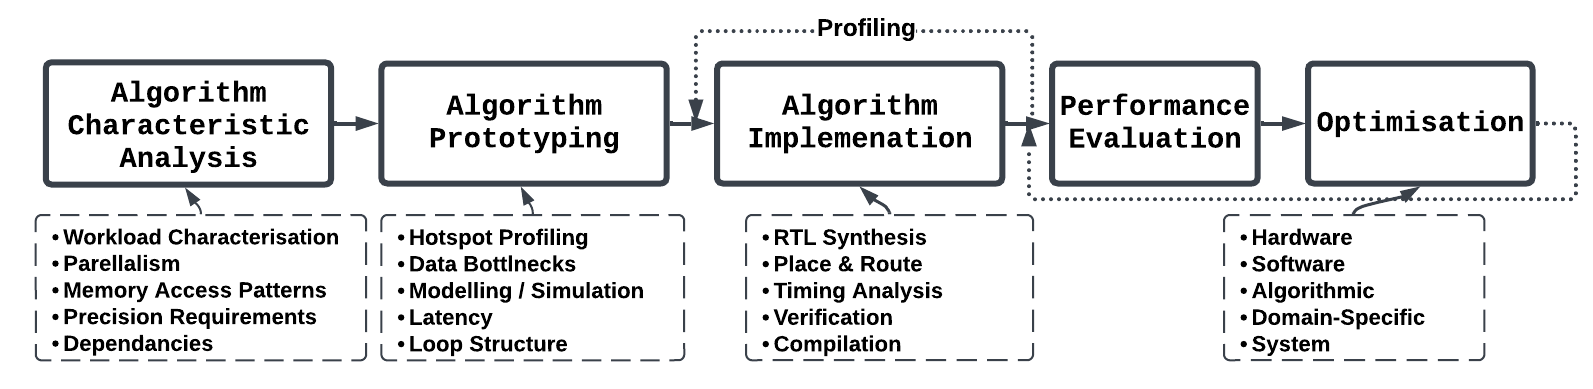
\includegraphics[width=\linewidth]{Images/Bencmark Flow.png}
\caption[Framework Pipeline]{Framework Pipeline for Heterogeneous Image Processing }
\label{fig:FrameworkFlow}
\end{figure}

Therefore, To effectively exploit the power of heterogeneous architectures, a robust development flow is crucial. Such a workflow not only aids in pinpointing the optimal architecture but also streamlines the entire development process. As depicted in \Fig{FrameworkFlow}, a comprehensive heterogeneous development pipeline describes a systematic and standardised approach for implementation. This structured flow ensures that developers can seamlessly integrate various computational resources, leverage specialised hardware capabilities, and achieve optimal performance across multiple platforms.

\textbf{Characteristic Analysis:} The first stage involves identifying certain properties of an algorithm discussed in \ref{sec:framework} and building a model of data, which helps find suitable architectures. Starting with workload characterisation provides a comprehensive overview of the algorithm's computational and data demands, potentially giving insight into areas where algorithms can be partitioned. Specific algorithms require higher precision, which can impact the choice of the target architecture. However, trading off accuracy for speed is a potential opportunity. Memory access patterns significantly affect cache utilisation and memory latency. It's important to recognise an algorithm's parallelism potential while being aware of data dependencies. Moreover, optimising memory access patterns to align with the cache hierarchy can reduce latency and enhance memory throughput. Furthermore, adapting algorithms to harness specific hardware features, such as GPU threads, FPGA pipelines, or TPU matrix multiply units.


\textbf{Prototyping:} 
This stage involves prototyping designs to identify the initial performance of an architecture to establish a baseline benchmark. Profiling code is done to identify performance bottlenecks, which offers valuable insights into areas suitable for performance enhancement across various architectures. Profiling aims to uncover the 'hotspots,' sections of code where execution time and resource consumption are disproportionately high. In addition, identifying task, data parallelism or pipelining opportunities which benefit certain accelerators. It is essential to pinpoint potential latency issues, both in I/O operations and within memory, which can arise from slow data transfers or inefficient data handling. Identifying loop structures is important for performance; branching within loops in parallel or pipelined processors can negatively affect performance. This is because branching can lead to divergence, where different execution paths are taken simultaneously, causing processing cores to remain idle. Loop unrolling is a common optimisation technique that can mitigate the effects of branching by increasing the number of operations in each loop iteration, reducing the loop's overhead. However, if a loop cannot be unrolled or tiled, it may be more efficient to execute the algorithm on a higher clocked sequential core, which can handle branching.


\textbf{Implementation:} 
After selecting the appropriate architecture for an algorithm, the next step involves its implementation. Depending on the chosen accelerator, this process may entail simulating and synthesising designs and conducting thorough verification. Finally, timing analysis involves evaluating the propagation delays of signals through the circuit's logic gates and interconnects to ensure they meet the constraints set by the clock cycle time. This helps in detecting and addressing potential timing violations. General-purpose architectures will use compilation methods to high-level code into machine-level instructions tailored for the instruction driven accelerators.

\textbf{Evaluation \& Optimisation:}
Post-implementation, performance tuning and optimisation techniques are applied to ensure the algorithm runs efficiently, maximising the hardware's potential. Optimisations can be grouped into four categories: hardware, software, domain-specific and algorithmic. Hardware optimisations involve fine-tuning specific hardware configurations or datatypes such as quantisation or bit-width adjustments. Software optimisations are usually applied at the code level either manually or automatically by compilers. These techniques can include inlining, dead code elimination, and vectorization. Domain-specific is tailored for specific application areas such as downsampling or separable filters. Lastly, algorithmic focus on mathematical refinement to reduce complexity and use more efficient data structures. It's also necessary to validate the implementation against reference data-sets to ensure functional correctness. Throughout this process, continuous profiling helps identify bottlenecks and areas for further optimisation. 




\section{Benchmarking Methodology}\label{sec:benchmark}
This section introduces two benchmarking strategies, micro and macro, each offering distinct approaches to evaluate accelerator performance. While micro-benchmarking focuses on assessing individual algorithms or pipelines, macro-benchmarking provides an overall view by analysing fundamental operations found in many algorithms within the ISP pipeline.

\subsection{Micro Benchmarking Algorithms}\label{Benchmarking Algorithms}
%-------------------------------------------
\begin{figure}[t]
\centering
  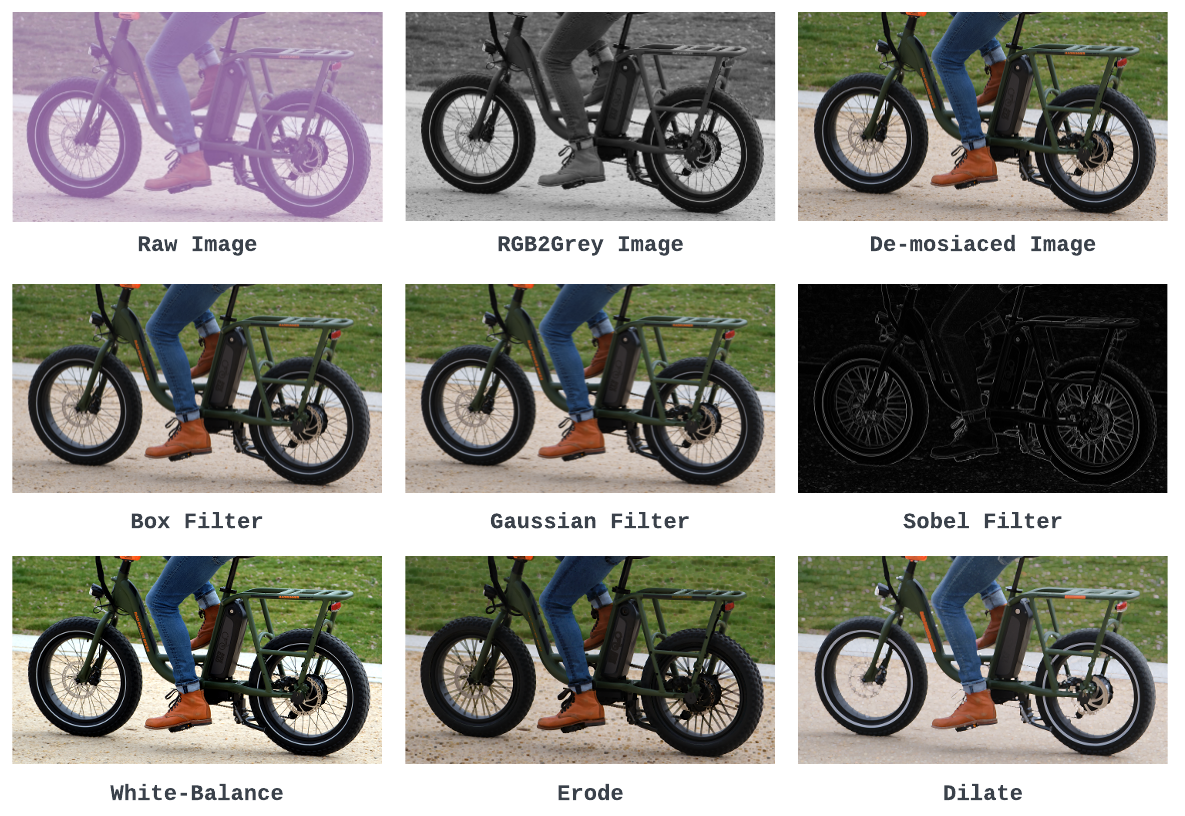
\includegraphics[width=\textwidth]{Images/Processed Images.png}
    \caption[Exemplar Image Pipelines]{Low to High Complexity Image Processing Algorithms in the ISP Pipeline}
    \label{fig:edge-detect} 
\end{figure}
%---------------------------------------------------------------

\begin{table}
\centering
\setlength{\extrarowheight}{0pt}
\addtolength{\extrarowheight}{\aboverulesep}
\addtolength{\extrarowheight}{\belowrulesep}
\setlength{\aboverulesep}{0pt}
\setlength{\belowrulesep}{0pt}
\caption{List of Implemented Image Processing \& Benchmarking Algorithms}
\label{tab:algorithms}
\resizebox{\linewidth}{!}{%
\begin{tabular}{c|c|c|c|c} 
\toprule
\rowcolor[rgb]{0.753,0.753,0.753} Algorithm & Complexity & Operator Group & Configuration & Description \\ 
\cmidrule{1-3}\cline{4-4}\cmidrule{5-5}
RGB2Grey & Low & Point Operations & \multicolumn{1}{l|}{\begin{tabular}[c]{@{}l@{}}R:0.299 G:0.587\\B:0.114\end{tabular}} & Convert RGB image to greyscale \\ 
\hline
Resizing & Low & Geometric Transformation & 2.5x Upsampling & Change image dimensions by interpolation \\ 
\hline
Image Addition & Low & Point Operations & \textasciitilde{} & Add two images pixel-wise \\ 
\hline
Image Subtraction & Low & Point Operations & \textasciitilde{} & Subtract one image from another pixel-wise \\ 
\hline
Gamma Correction & Low & Linear Filter & \gamma = 2.2 & Adjust pixel intensities using gamma values \\ 
\hline
Linearization & Medium & Point Operations & \textasciitilde{} & Correct non-linear sensor response \\ 
\hline
Erode & Medium & Morphological Operations & 5x5 & Erode image regions \\ 
\hline
Dilate & Medium & Morphological Operations & 5x5 & Dilate image regions \\ 
\hline
Box Filter & Medium & Linear Filter & 5x5 & Apply simple box averaging \\ 
\hline
Gaussian Filter & Medium & Linear Filter & 5x5 & Apply Gaussian blurring \\ 
\hline
Sobel Filter & Medium & Non-linear Filter & 7x7 & Detect edges using Sobel operator \\ 
\hline
Median & Medium & Non-linear Filter & 5x5 & Replaces each pixel value with the median value \\ 
\hline
White Balance & Medium & Linear 

Filter & Gray World  & Adjust color balance in images \\ 
\hline
GEMM & Medium & Fundamental & N=4096 & General Matrix Multiply (GEMM) operation \\ 
\hline
FFT (DFT) & Medium & Fundamental & \begin{tabular}[c]{@{}c@{}}radix-2 / R2C\\Zero Padding\end{tabular} & Compute Fast Fourier Transform of signals \\ 
\hline
STREAM & Medium & Fundamental & N=1 \times 10^7 & Evaluate memory bandwidth and latency \\ 
\hline
Demosaicing & Medium & Non-linear Filter & \begin{tabular}[c]{@{}c@{}}Bilinear\\Interpolation\end{tabular} & Convert Bayer-pattern image to RGB \\ 
\hline
SIFT & High & Feature Extraction & 2 Octave 4 Scale & Scale-Invariant Feature Transform for image matching \\ 
\hline
\begin{tabular}[c]{@{}c@{}}CNN (Classification)\\\end{tabular} & High & Deep Learning & \begin{tabular}[c]{@{}c@{}}ResNet18 \& \\MobileNetV2\end{tabular} & Feature Extraction and Classification using Neural Networks \\
\bottomrule
\end{tabular}
}
\end{table}
Image processing pipelines contain many operations varying in complexity. For a comprehensive set of results, many popular individual ISP algorithms are chosen to be benchmarked, listed in \Tab{algorithms} and visually shown in \Fig{edge-detect}. The algorithms, \textit{Addition},  \textit{Subtraction}, \textit{Erode}, \textit{Dilate}, \textit{Box Filter}, \textit{Gamma Correction}, \textit{Linearization}, and \textit{Demosaicing} are chosen because they represent foundational operations in image processing. These algorithms exhibit diverse memory access patterns, computational intensities, and parallelism levels. Their inclusion ensures a comprehensive evaluation of an architecture's capability to handle point-wise and neighbourhood operations.


\subsubsection{Complete Imaging Pipelines}
\begin{figure}[t]
\centering
  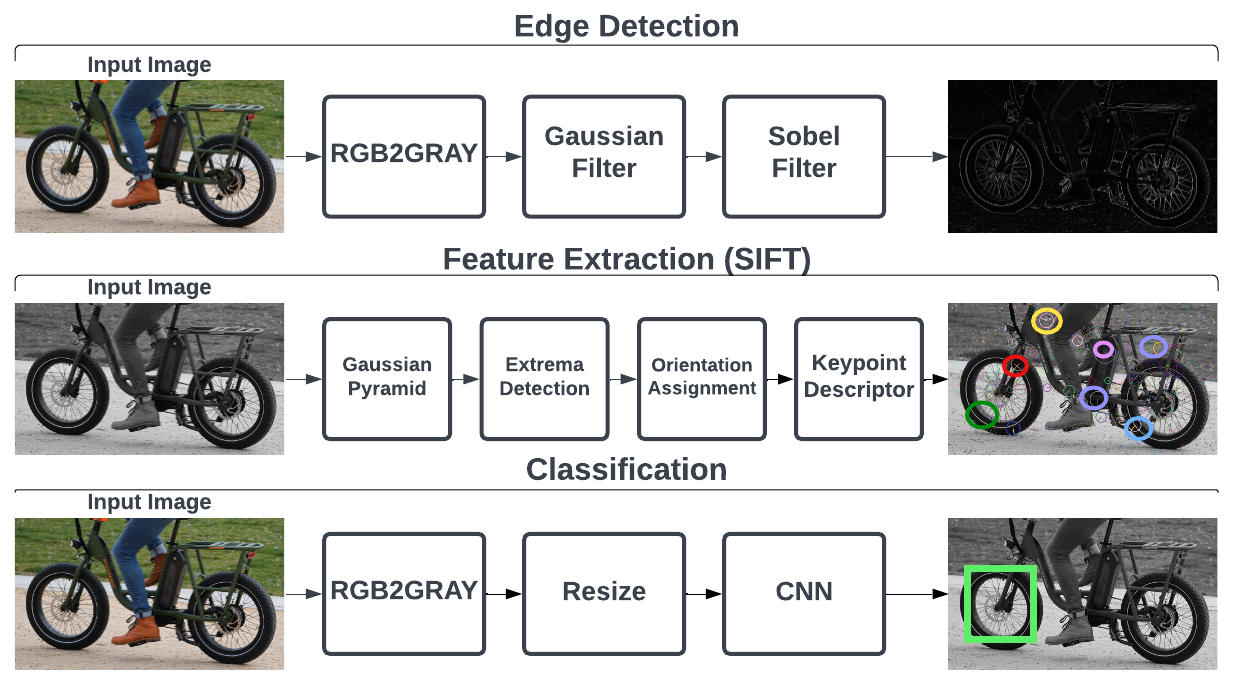
\includegraphics[width=\textwidth]{Images/PopularPipeline.png}
    \caption[Exemplar Image Pipelines]{Exemplar Image Pipelines Benchmarked on each Architecture. }
    \label{fig:completepipelines} 
\end{figure}

Vision applications usually do not consist of one algorithm but contain many pipelined together to form a complete system. In developing the proposed framework, three exemplars were selected: 1) \textit{Edge Detection}, 2) \textit{Feature Extraction (SIFT)}~\cite{Low99} and 3) Classification, representing low to high-level complexity shown in \Fig{completepipelines}. They are partitioned into nine sub-algorithms, namely, \textit{RGB2Grey}, \textit{Gaussian Filter}, \textit{Sobel Filter},  \textit{Gaussian Pyramid}, \textit{Extrema Detection}, \textit{Orientation Assignment}, \textit{Descriptor Generation}, \textit{Resize}, and \textit{CNN}. The sub-algorithms are common building blocks of many other image processing algorithms with varying complexity and therefore are good candidates for benchmarking. For example, \textit{Gaussian Pyramid} is useful for analysis across different spatial scales and \textit{Extrema Detection} operations are often used in corner detection and image blending algorithms.

The first pipeline is the edge detection pipeline, designed to identify and emphasise edges within images. It starts with the conversion of RGB colour information into greyscale, a method aimed at reducing redundant processing. Following this, Gaussian filtering is used to achieve image smoothing and noise reduction, essential for accurate edge detection. The Sobel edge detection algorithm, serving as the final stage within this pipeline, detects edges by highlighting abrupt changes in pixel intensities.

The feature extraction pipeline captures important features present within images. The first step in the pipeline involves the construction of a Gaussian pyramid, accomplished by generating multiple versions of the input image through Gaussian filtering and downsampling. This pyramid plays a critical role in identifying features across varying scales. Subsequently, extremum detection is executed, facilitating the identification of keypoints or points of interest within the image. These keypoints serve as reference points for subsequent analysis and interpretation. Grayscale images is used as a input for their simplicity in processing and their robustness to changes in illumination.

The classification pipeline can be found in many deep learning based applications, including vision. It begins with the conversion of RGB to greyscale and subsequently, the image resizing operation is performed to standardise dimensions, ensuring compatibility with the CNN architecture. The final stage involves the application of the CNN algorithm, a state-of-the-art deep learning technique known for its proficiency in tasks related to image classification, object detection, and segmentation.


\subsection{Macro Benchmarking Algorithms}
Many image processing algorithms share foundational operations, which can be used to benchmark accelerators to gain better insight. This section reviews a range of algorithms and their properties that make it an ideal case study for evaluation.


\subsubsection{Sustainable Memory Bandwidth in High Performance Computers}
 Stream memory benchmark\cite{Macc06} (STREAM) is a widely used performance evaluation tool for measuring memory bandwidth in computer systems. It assesses the speed at which a system can read and write data to memory. The benchmark primarily focuses on four memory access patterns: Copy, Scale, Add, and Triad. In the Copy pattern, data is read from one memory location and written to another. The Scale pattern involves reading data, scaling it by a constant, and writing it to a different memory location. The Add pattern reads two arrays, adds corresponding elements, and writes the result to a third array. Finally, the Triad pattern combines scaling and addition operations. The benchmark generates a set of memory performance metrics, including the memory bandwidth, calculated as the amount of data transferred per unit time, typically in gigabytes per second (GB/s).
 The memory bandwidth (B) can be calculated using the following equation:
\begin{equation}
 B = \frac{N \times S}{t} 
\end{equation}

 where $N$ is the number of data elements accessed in the memory, $S$ is the size of each data element in bytes, and $t$ is the time taken to complete the memory operation in seconds. This equation gives us the memory bandwidth in bytes per second. Image processing is very memory-intensive due to the large amounts of data associated with higher resolution images and the need for frequent data access during processing. Each pixel requires multiple bytes of storage, and when processing, these pixels often need to be accessed multiple times, especially in operations like convolution, filtering, or transformations. The STREAM benchmark becomes invaluable in this context, as it provides insights into how efficiently an architecture can handle the memory demands of image processing tasks.

 \subsubsection{Fast Fourier Transform}
 Fast Fourier Transform (FFT) is an algorithm that finds extensive applications in signal processing, image analysis, and various fields where frequency domain analysis is essential. In image processing, FFT is particularly valuable for transforming an image from its spatial domain representation to its frequency domain representation. This transformation enables the identification of various frequency components present in an image, offering insights into patterns, textures, and other intricate details that may not be as evident in the spatial domain.

The FFT algorithm computes the Discrete Fourier Transform (DFT) of a signal in an efficient manner, reducing the computational complexity from $O(n^2)$ to $O(n \log (n))$, where $n$ is the number of data points in the signal. In the case of a 2D image, the FFT operation involves applying the DFT algorithm separately to both the rows and columns of the image's pixel values. The 2D FFT of an image $I(x, y)$ is expressed as:

\begin{equation}
F(u, v) = \sum_{x=0}^{N-1} \sum_{y=0}^{M-1} I(x, y) e^{-j 2 \pi \left(\frac{u x}{N} + \frac{v y}{M}\right)}
\end{equation}

Here, $F(u, v)$ represents the frequency components in the transformed image, N is the number of pixels along the x-axis, $M$ is the number of pixels along the y-axis, and $(u, v)$ are the spatial frequency coordinates in the frequency domain.

The resulting 2D FFT representation provides valuable information about the image's frequency content. Low-frequency components (corresponding to slow changes in intensity) are typically located near the centre of the frequency domain representation. High-frequency components (corresponding to rapid changes in intensity, edges, and textures) tend to be found towards the corners. By analysing this transformed image, practitioners can perform tasks like filtering, denoising, compression, and other frequency-based manipulations to enhance or extract specific features from the original image.



\subsubsection{Convolution (Matrix Multiply)}
The two most common methods for convolution are general matrix multiply (GEMM) and direct convolution. GEMM-based convolution relies on the \textit{im2col} algorithm\cite{CheKumPur06}, which results in a large memory footprint and reduced performance. Alternatively, direct convolution has a lower memory footprint but the performance is reduced due to the irregular memory access patterns. GEMM can be  can be expressed through \Eq{GEMM}:

\begin{equation}\label{eq:GEMM}
C_{ij} = \sum_{k=1}^{K} A_{ik} \cdot B_{kj}
\end{equation}

Here, $C_{ij}$ refers to the element positioned at row $i$ and column $j$ within the resultant matrix $C$, $A_{ik}$ signifies the element situated at row $i$ and column $k$ in matrix $A$, and $B_{kj}$ represents the element located at row k and column $j$ in matrix $B$. The summation spans across the index $k$ from 1 to $K$, where $K$ corresponds to the number of columns in matrix $A$ (which should equivalently match the number of rows in matrix BB for accurate multiplication). This equation forms the core operation underlying the GEMM benchmark, which orchestrates the calculation of the matrix product between $A$ and $B$ to yield matrix $C$.

GEMM is found in image processing tasks that require matrix operations. For example, convolutional neural networks (CNNs) extensively use matrix multiplications for convolutional layers, and GEMM's efficiency and parallelism make it highly useful for accelerating these operations. Additionally, transformations, filters, and image manipulations often involve matrix operations, and therefore GEMM's optimised implementations can significantly enhance the performance of image processing algorithms. 


\subsection{Performance Metrics}
This section focuses on evaluating implemented image processing algorithms using two key metrics: execution time and power consumption. The analysis provides insights into the strengths and limitations of the image processing algorithms on a heterogeneous architecture.

% \begin{figure}[H]
%     \centering
%     \begin{tabular}{cc}
%     \resizebox{0.5\linewidth}{!}{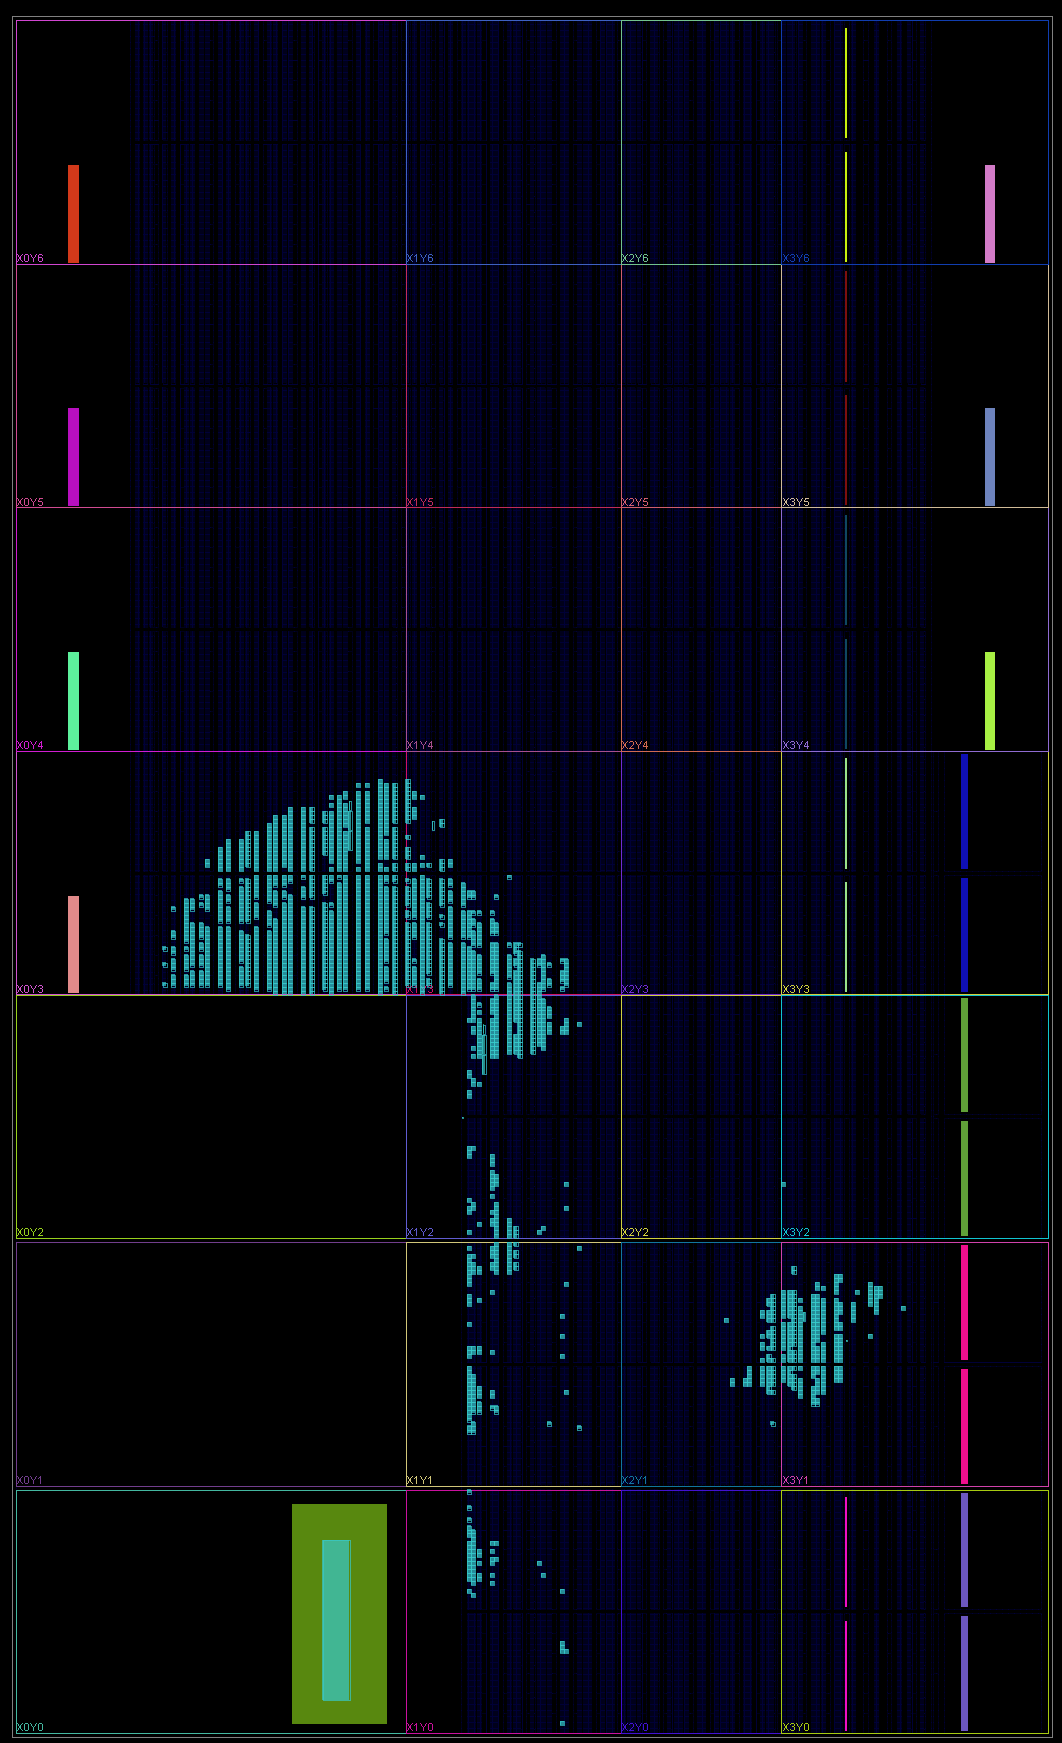
\includegraphics{Images/GaussianBlur.png}} &
%     \resizebox{0.5\linewidth}{!}{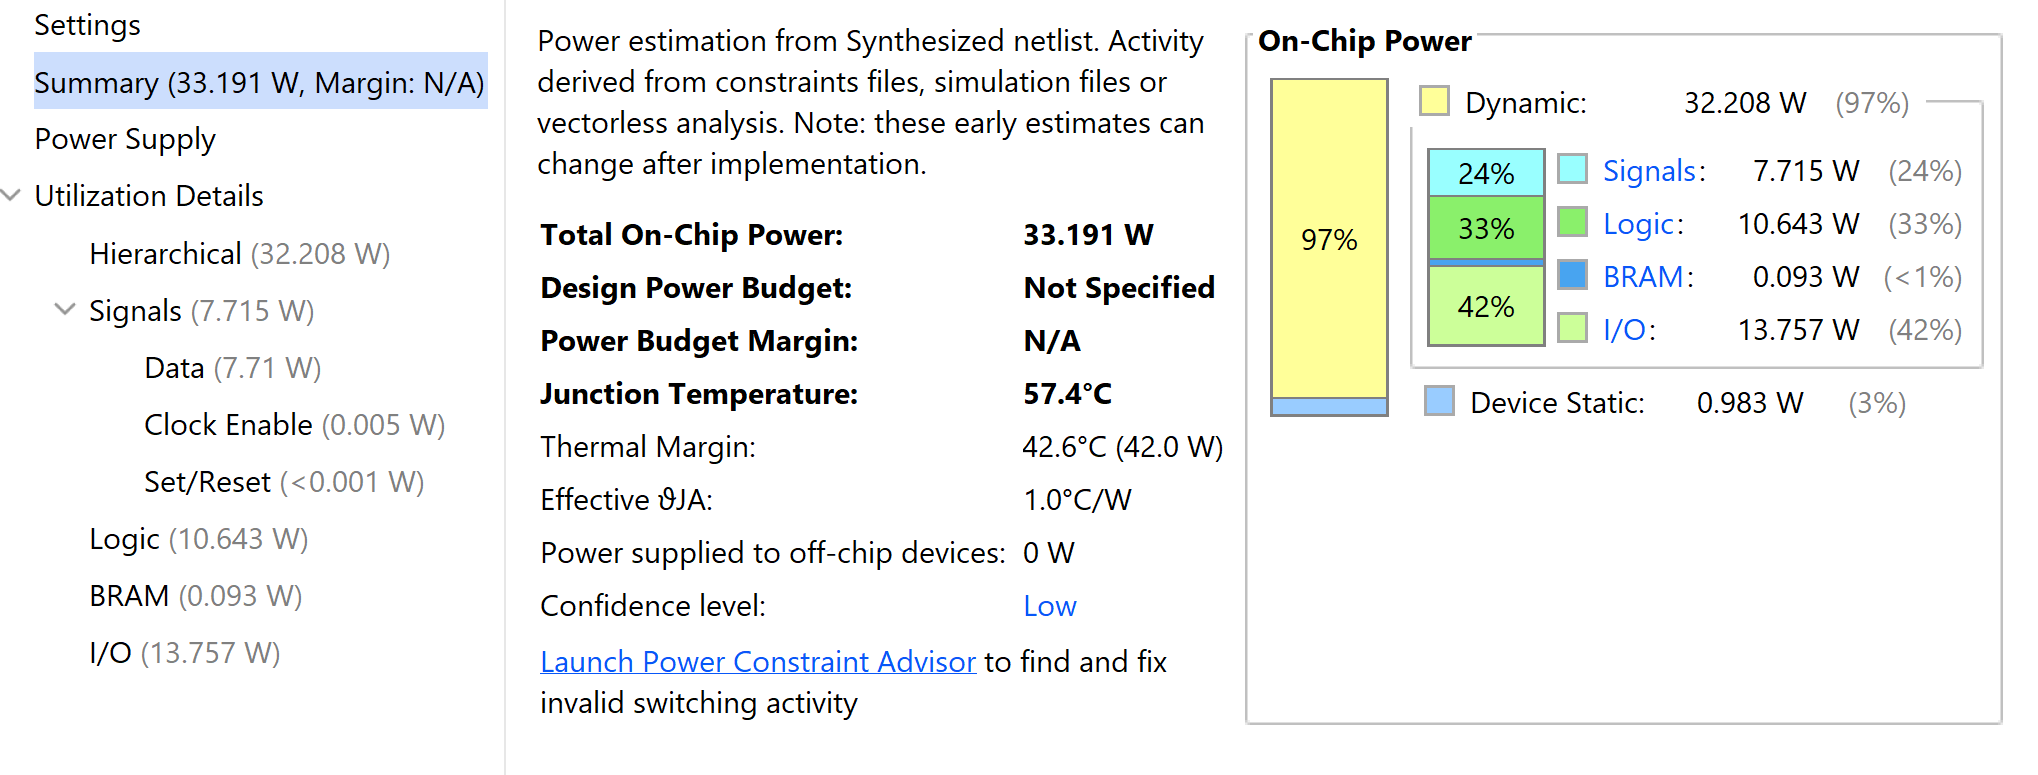
\includegraphics{Images/PowerUsageUsage.png}} \\
%     (a) & (b) \\
%     \end{tabular}
%     \caption{a) Resource Usage  b) Vivado Power Analyser}
%     \label{fig:CMOS Image Sensor}
% \end{figure}

\subsubsection{Execution Time}
In evaluating the performance of image processing algorithms, precise time measurements are essential to capture the subtle differences across hardware platforms. For the CPU, the C++ standard library's $high\_resolution\_clock$ is employed, offering a fine-grained temporal resolution suitable for capturing in microseconds. This method involves marking the start and end times surrounding the algorithm's execution and computing the difference to determine the elapsed time. On the GPU side, CUDA events were utilised to measure the time taken for the algorithms to run. CUDA events are specifically designed to capture start and end times in a GPU's environment, ensuring accurate timing measurements that account for the asynchronous nature of GPU operations. Irrelevant processes are stopped within the operating system to prevent interference during the timing measurement. For the FPGA evaluations, the behavioural simulation timing feature of the Vivado software is used. This tool provides a detailed timing analysis, simulating how the algorithm would perform on the FPGA, thereby offering insights into its expected real-world performance. The  implementations are written in C/C++/Verilog and uses the time function built into Linux and system performance monitor to measure the runtime of CPU/GPU/FPGA.

\subsubsection{Power Consumption}
Accurate power estimation is always challenging for software tools. However, systematic steps are taken to minimise assumptions for better accuracy. The approach used to measure the power consumption for the CPU and GPU is obtained by using \textit{HWMonitor} software. The power is initially measured to determine the average base operating power. Then, each algorithm is executed multiple times, and the power is measured during algorithm runtime. The FPGA on-chip power consumption is measured using the reports from the power analyser feature integrated into Vivado Design Suite. The heterogeneous implementation power consumption is calculated using both \textit{HWMonitor} and Xilinx's System Monitor IP. Static power consumption, refers to the constant energy usage of a device when it's idle, whereas dynamic power consumption varies based on the workload or activity levels, resulting in fluctuations in energy usage



\subsection{Measurement Environments}

% \begin{table}[tb]
%     \caption{Implementation environment summary.}
%     \label{tab:PlatformSummary}
%     \centering
%     \resizebox{0.7\columnwidth}{!}{%
%     \begin{tabular}{c|c|c|c|c}
%     \toprule
%         Platform &Flexibility & Language & Library      & Programmability \\ \midrule
%         CPU      & Flexible            & C++      & OpenCV 4.3.0 & Easy         \\ \midrule
%         GPU      & Flexible            & C++      & OpenCV (CUDA) & Easy        \\ \midrule
%         FPGA     & Inflexible          & C++ (HLS) &     xfOpenCV    & Medium   \\ \midrule
%         FPGA     & Inflexible          & Verilog  & None   & Difficult   \\ \bottomrule
%     \end{tabular}
%     }
% \end{table}
%---------------------------------

%--------------------------------------------------
%\begin{table}[tb]
%\caption{Hardware Environment} \label{tab:HWEnvironment}
%\centering
%\resizebox{0.7\columnwidth}{!}{%
%\begin{tabular}{l|l}
%\toprule
%CPU & \begin{tabular}[c]{@{}l@{}}AMD 5900x  (4.8 GHz, 12 Core, 24 Threads, 70 MB cache)\end{tabular} \\ \midrule
%GPU & \begin{tabular}[c]{@{}l@{}}Nvidia GTX 3070 (1730 MHz, 5888 CUDA cores)\end{tabular}            \\ \midrule
%FPGA & \begin{tabular}[c]{@{}l@{}}Xilinx Zynq UltraScale+  MPSoC ZCU102 16+nm (300Mhz)\end{tabular} \\ \bottomrule
%\end{tabular}.
%}
%\end{table}
%----------- 
While FPGA can provide an accurate execution time in the simulation mode, the same is not true for the CPU/GPU accelerators, as there might be other software (including part of the operating system) competing for compute resources. To mitigate this, the execution time for each bench-marked algorithm is measured as the average of 1,000 iterations on CPU/GPU and closing all other non-core application processes before execution. The Nvidia (CUDA) GPU also has an initialisation time often associated with setting up the GPU context and memory allocations, can be significant, especially for smaller tasks. The initialisation time is recorded for both with and without.




%--------------------------------------------------
\begin{table}[tb]
\centering
\setlength{\extrarowheight}{0pt}
\addtolength{\extrarowheight}{\aboverulesep}
\addtolength{\extrarowheight}{\belowrulesep}
\setlength{\aboverulesep}{0pt}
\setlength{\belowrulesep}{0pt}
\caption[Hardware/Software Environment Summary]{Summary: Hardware/Software Environment, Measurement Tools.}
\label{tab:CombinedEnvironment}
\arrayrulecolor{black}
\resizebox{\linewidth}{!}{%
\begin{tabular}{c|c|c|c|c|c|c} 
\toprule
\rowcolor[rgb]{0.753,0.753,0.753} {\cellcolor[rgb]{0.753,0.753,0.753}} & \multicolumn{2}{c|}{\textbf{Hardware}} & {\cellcolor[rgb]{0.753,0.753,0.753}} & {\cellcolor[rgb]{0.753,0.753,0.753}} & {\cellcolor[rgb]{0.753,0.753,0.753}} & {\cellcolor[rgb]{0.753,0.753,0.753}} \\ 
\hhline{>{\arrayrulecolor[rgb]{0.753,0.753,0.753}}->{\arrayrulecolor{black}}|-|-|>{\arrayrulecolor[rgb]{0.753,0.753,0.753}}->{\arrayrulecolor{black}}|>{\arrayrulecolor[rgb]{0.753,0.753,0.753}}->{\arrayrulecolor{black}}|>{\arrayrulecolor[rgb]{0.753,0.753,0.753}}->{\arrayrulecolor{black}}|>{\arrayrulecolor[rgb]{0.753,0.753,0.753}}-}
\rowcolor[rgb]{0.753,0.753,0.753} \multirow{-2}{*}{{\cellcolor[rgb]{0.753,0.753,0.753}}\textbf{Architecture}} & \textbf{Model} & \textbf{Clock} & \multirow{-2}{*}{{\cellcolor[rgb]{0.753,0.753,0.753}}\begin{tabular}[c]{@{}>{\cellcolor[rgb]{0.753,0.753,0.753}}c@{}}\textbf{Software/}\\\textbf{Libraries }\end{tabular}} & \multirow{-2}{*}{{\cellcolor[rgb]{0.753,0.753,0.753}}\begin{tabular}[c]{@{}>{\cellcolor[rgb]{0.753,0.753,0.753}}c@{}}\textbf{Power}\\\textbf{ Measurement}\end{tabular}} & \multirow{-2}{*}{{\cellcolor[rgb]{0.753,0.753,0.753}}\textbf{Language}} & \multirow{-2}{*}{{\cellcolor[rgb]{0.753,0.753,0.753}}\textbf{Programmability}} \\ 
\arrayrulecolor{black}\cmidrule{1-3}\cline{4-4}\cmidrule{5-7}
CPU & \begin{tabular}[c]{@{}c@{}}AMD \\5900x\end{tabular} & 4.8 GHz & \begin{tabular}[c]{@{}c@{}}Pytorch 2.0\cite{Pytorch} / \\OpenCV\cite{opencv_library}\end{tabular} & HWMonitor\cite{cpuid} & C++ & Easy \\ 
\cmidrule{1-1}\cline{2-7}
GPU & \begin{tabular}[c]{@{}c@{}}Nvidia \\GTX 3070\end{tabular} & 1730 MHz & \begin{tabular}[c]{@{}c@{}}Pytorch 2.0 / \\OpenCV\end{tabular} & Nvidia-smi\cite{Nvidiasmi} & C++ & Easy \\ 
\cmidrule{1-2}\cline{3-7}
FPGA (HLS) & \begin{tabular}[c]{@{}c@{}}Xilinx \\ZCU102\end{tabular} & 300Mhz & Vitis 2020.2 & \begin{tabular}[c]{@{}c@{}}MaxPower-tool\cite{XButil} / \\Power Analyser\end{tabular} & C++ & Medium \\ 
\cmidrule{1-2}\cline{3-7}
FPGA & \begin{tabular}[c]{@{}c@{}}Xilinx \\ZCU102\end{tabular} & 300Mhz & Vivado 2022.2 & \begin{tabular}[c]{@{}c@{}}MaxPower-tool / \\Power Analyser\end{tabular} & Verilog & Difficult \\
\bottomrule
\end{tabular}
}
\end{table}
%--------------------------------------------------

\noi\textbf{Software \& Hardware Environments:}
\textit{OpenCV} and \textit{Pytorch} library is used to implement image processing algorithms and CNNs on CPU and GPU platforms. The FPGA implementation is written in Verilog, using Vivado Design Suite 2019.2. Additionally, for comparison purposes, implementation was done with high-level synthesis (HLS) code using Xilinx Vitis 2019.2. Programmability and flexibility vary across architectures shown in \Tab{CombinedEnvironment}; CPUs and GPUs are general-purpose, which makes them highly programmable for a wide range of tasks, with languages like C++ being commonly used. FPGAs are more inflexible since significant time is needed to change implementation designs and are typically crafted in hardware descriptor languages such as Verilog. The hardware setup consists of a desktop PC running a Linux operating system, with a discrete GPU and FPGA connected via a high throughput PCIe interface to reduce data latency. 

\subsection{Measurement Approach}\label{sec:measurementApproach}
The algorithms are implemented individually on each hardware and then combined to create the combined pipeline. For a fair comparison, open-sourced (OpenCV) and CNN libraries(Pytorch) were employed, which are highly optimised for their respective architectures. This is with exception of the Verilog implementations that were developed manually. The parameter for each algorithms used float precision and $5\times5$ kernel size. During the benchmarking, for consistency, an uncompressed $8$ bit $1920 \times 1080$ greyscale (Colour for \textit{RGB2Gray} algorithm) bitmap image for all experiments and a bayerRAW equivalent for \textit{Demoasiacing} algorithm.

We provide multiple performance indicators to compare between architectures. For each algorithm, the runtime is measured on each hardware to determine which accelerator executed the operation in the least amount of time. The results from the runtimes are used to calculate the estimated throughput using~\Eq{flop}. The clock cycles per operation (CPO) in \Eq{ClockComplete} gives insight into the average number of cycles required to execute an instruction. To have a fair comparison across the target hardware, the energy per operation is normalised using \Eq{energyepo}:
%-------------Performance Metric Equations----------
\begin{equation}
\text{Throughput} = \frac{N}{t} \label{eq:flop}
\end{equation}

\begin{equation}
\text{CPO} = \frac{f \times t}{N} \label{eq:ClockComplete}
\end{equation}

\begin{equation}
\text{EPO} = \frac{P \times t}{N} \label{eq:energyepo}
\end{equation}

In these equations, $N$ denotes the number of operations performed and  $t$ signifies the runtime of the computational task in seconds. $f$ represents the frequency of the processing unit in hertz, and $P$ is power consumption in watts.




% The algorithms are implemented individually on each hardware and then combined to create the combined pipeline. For a fair comparison, open-sourced (OpenCV) and CNN libraries were employed, which are highly optimised for their respective architectures. This is with exception of the Verilog implementations that were developed manually. During the benchmarking, for consistency, an uncompressed $8$ bit $1920 \times 1080$ greyscale (Colour for \textit{RGB2Gray} algorithm) bitmap image for all experiments and a bayerRAW equivalent for \textit{Demoasiacing} algorithm.

% We provide multiple performance indicators to compare between architectures. For each algorithm, the runtime is measured on each hardware to determine which accelerator executed the operation in the least amount of time. The results from the runtimes are used to calculate the estimated throughput using~\Eq{flop}. The clock cycles per operation (CPO) in \Eq{ClockComplete} gives insight into the average number of cycles required to execute an instruction. To have a fair comparison across the target hardware, the energy per operation is normalised using \Eq{energyepo}:
% %-------------Performance Metric Equations----------
% \begin{align}
% \text{Throughput} &= {(\text{Number of Operations})}/{\text{Runtime}}. \label{eq:flop} \\
% \text{CPO}  &= {(\text{Frequency}*\text{Runtime})}/{\text{Operation}}. \label{eq:ClockComplete} \\
% \text{EPO} &= {(\text{Power} * \text{Runtime})}/{\text{Operation}}. \label{eq:energyepo}
% \end{align} 

% \Eq{eq:runtimeconsumption}
% \begin{equation}\label{eq:runtimeconsumption}
% Runtime = \sum_{i=1}^{n} t_{hw_i} = t_{hw_1} + t_{hw_2} + \dots + t_{hw_n}
% \end{equation}

% \Eq{powerconsumptionHA} quantifies the energy consumption in joules of individual hardware components within a heterogeneous architecture, normalised by their respective runtimes. In this equation, \(E_{hw_i}\) represents the energy consumption of the \(i^{\text{th}}\) hardware component, while \(t_{hw_i}\) denotes its runtime. This formula provides a comprehensive measure of power consumption across diverse hardware elements in a heterogeneous computing environment.


% \begin{equation}\label{eq:powerconsumptionHA}
% Energy \, Consumption = \sum_{i=1}^{n} \frac{E_{hw_i}}{t_{hw_i}} = \frac{E_{hw_1}}{t_{hw_1}} + \frac{E_{hw_2}}{t_{hw_2}} + \dots + \frac{E_{hw_n}}{t_{hw_n}}
% \end{equation}





\section{Experiments, Results \& Discussion}\label{sec:result}
This section presents the bench-marked results of each algorithm described in~\ref{sec:benchmark} and an in-depth discussion. The section is divided into two parts, which include the runtime, power consumption, EPO and throughput results for individual ISP algorithms and combined exemplar pipelines.


\subsection{Individual ISP Algorithms}


%--------------Individual Runtime--------------
\begin{figure}[t]
    \centering
\resizebox{\columnwidth}{!}{\pgfplotsset{width=\textwidth,compat=1.3}
\begin{tikzpicture}
    \begin{axis}[
        width  = \textwidth,
        major x tick style = transparent,
        ybar=2*\pgflinewidth,
        ymin=0,ymax=100,
        bar width=4.1pt,
        enlarge y limits={upper=0.15},
        legend image code/.code={\draw[#1, draw=none] (0cm,-0.1cm) rectangle (0.3cm,0.1cm);
                },
        ymajorgrids = true,
        ylabel = {Execution Time (ms)},
        symbolic x coords={CPU,GPU,FPGA,HLS},
        xtick = data,
        nodes near coords,
        nodes near coords style={font=\tiny, anchor=west,rotate=90,inner xsep=0.5pt,black},
        scaled y ticks = false,
        enlarge x limits=0.15,
        legend cell align=left,
           enlarge y limits={upper=0.15},
    legend style={at={(0.17,0.88)},
                   anchor=west,legend columns=4, font=\small},
    ]
        \addplot[style={blue,fill=blue!60}]
            coordinates {(CPU, 0.75) (GPU,0.45) (FPGA,0.40)(HLS,0.54)}; % RGB2GRAY
        \addplot[style={darkcandyapplered,fill=darkcandyapplered}]
             coordinates {(CPU,3.5) (GPU,0.28) (FPGA,0.25)(HLS,0.31)}; % Gaussian
        \addplot[style={forestgreen,fill=forestgreen}]
             coordinates {(CPU,15.1) (GPU,9.88) (FPGA,8.23)(HLS,9.65)}; % Box
        \addplot[style={gray,fill=gray}]
             coordinates {(CPU,105) (GPU,64) (FPGA,71)(HLS,77)}; % Median
        \addplot[style={pastelorange,fill=pastelorange}]
             coordinates {(CPU,25.7) (GPU,0.51) (FPGA,1.2)(HLS,2.53)}; % Sobel
        \addplot[style={oorange,fill=oorange}]
             coordinates {(CPU,1.6) (GPU,0.3) (FPGA,0.24)(HLS,0.44)}; % resize
        \addplot[style={purple,fill=purple}]
             coordinates {(CPU,2.6) (GPU,0.30) (FPGA,0.25)(HLS,0.88)}; % image add
        \addplot[style={richlavender,fill=richlavender}]
             coordinates {(CPU,2.5) (GPU,0.18) (FPGA,0.18)(HLS,0.24)}; % image subtract
        \addplot[style={teal,fill=teal}]
             coordinates {(CPU,9.2) (GPU,5.5) (FPGA,6.6)(HLS,7.1)}; % erode
        \addplot[style={ppink,fill=ppink}]
             coordinates {(CPU,9.3) (GPU,5.7) (FPGA,6.8)(HLS,7.1)}; % dilate
        \addplot[style={bbrown,fill=bbrown}]
             coordinates {(CPU,43) (GPU,7) (FPGA,14)(HLS,23)};  % Gamma           
        \addplot[style={cyan,fill=cyan}]
             coordinates {(CPU,10.8) (GPU,0.25) (FPGA,0.20)(HLS,0.31)}; % Placeholder for Linearization
        \addplot[style={magenta,fill=magenta}]
             coordinates {(CPU,21.6) (GPU,0.19) (FPGA,0.28)(HLS,0.55)}; % Placeholder for White Balance
        \addplot[style={peridot,fill=peridot}]
             coordinates {(CPU,32) (GPU,0.44) (FPGA,1.1)(HLS,1.7)}; % GEMM
        \addplot[style={wenge,fill=wenge}]
             coordinates {(CPU,44) (GPU,24) (FPGA,18)(HLS,20)}; % FFT
        \addplot[style={yellow-green,fill=yellow-green}]
             coordinates {(CPU,1.8) (GPU,1.1) (FPGA,1.4)(HLS,1.4)}; % STREAM
        \addplot[style={brown,fill=brown}]
             coordinates {(CPU,3.3) (GPU,0.87) (FPGA,1.24)(HLS,1.82)}; %Demosaicing
        \legend{R2G,Gaussian,Box, Median, Sobel,Resizing, Addition, Subtraction, Erode, Dilate, Gamma Corr., Linearization,White Balance,GEMM, FFT, STREAM, Demosaicing}
    \end{axis}
\end{tikzpicture}

%266}    
    \caption[Individual Algorithm Runtime]{{Execution times (milliseconds) for \textit{individual algorithms} found within imaging pipelines on each hardware architecture.}}
    \label{fig:OtherAlgorithmsExecutionTime}
\end{figure}
%-----------------------------------------------------

\Fig{OtherAlgorithmsExecutionTime} \& \Fig{CHAP1OtherAlgorithmsPower} plots the execution time (in milliseconds) and power consumption (in Watts) of the selected benchmarking image processing algorithms varying in complexity across different hardware architectures: CPU, GPU, FPGA, and high-level synthesis implementation on FPGA. The results reveal runtime variations among the architectures for each algorithm. Overall, the CPU performs competitively with the GPU, FPGA and HLS for lower complexity algorithms cases such as \textit{RGB2GRAY} algorithm, \textit{Addition}, and \textit{Subtraction}. It's evident that algorithms involving a small number of operations, such as colour channel conversion, do not require many computational cores to leverage parallelism or memory access requirements. However, the CPU's performance starts to decline as the complexity of the algorithms increases, as seen in cases like \textit{Sobel}, \textit{Gamma Correction}, \textit{GEMM}, and \textit{FFT}, where the large array processing capabilities offered by the GPU and FPGA become more prominent. On average, the CPU is $4.5\times$ and $4.35\times$ slower than the GPU and FPGA, respectively. 

%----------------Individual Power-----------------

\begin{figure}[t]
    \centering
\resizebox{\columnwidth}{!}{\pgfplotsset{width=\textwidth,compat=1.3}
\begin{tikzpicture}
    \begin{axis}[
        width  = \textwidth,
        major x tick style = transparent,
        ybar=2*\pgflinewidth,
        ymin=0,ymax=100,
        bar width=4.1pt,
        enlarge y limits={upper=0.15},
        legend image code/.code={\draw[#1, draw=none] (0cm,-0.1cm) rectangle (0.3cm,0.1cm);
                },
        ymajorgrids = true,
        ylabel = {Power Consumption (Watts)},
        symbolic x coords={CPU,GPU,FPGA,HLS},
        xtick = data,
        nodes near coords,
        nodes near coords style={font=\tiny, anchor=west,rotate=90,inner xsep=0.5pt,black},
        scaled y ticks = false,
        enlarge x limits=0.17,
        legend cell align=left,
           enlarge y limits={upper=0.15},
    legend style={at={(0.342,0.864)},
                   anchor=west,legend columns=3, font=\small},
    ]
        \addplot[style={blue,fill=blue}]
            coordinates {(CPU, 65) (GPU,32) (FPGA,20)(HLS,23)}; % RGB2GRAY
        \addplot[style={darkcandyapplered,fill=darkcandyapplered}]
             coordinates {(CPU,75) (GPU,36) (FPGA,26)(HLS,27)}; % Gaussian
        \addplot[style={forestgreen,fill=forestgreen}]
             coordinates {(CPU,82) (GPU,38) (FPGA,27)(HLS,30)}; % Box
        \addplot[style={gray,fill=gray}]
             coordinates {(CPU,102) (GPU,61) (FPGA,42)(HLS,48)}; % Median
        \addplot[style={pastelorange,fill=pastelorange}]
             coordinates {(CPU,85) (GPU,44) (FPGA,32)(HLS,33)}; % Sobel
        \addplot[style={oorange,fill=oorange}]
             coordinates {(CPU,73) (GPU,30) (FPGA,21)(HLS,24)}; % resize
        \addplot[style={purple,fill=purple}]
             coordinates {(CPU,70) (GPU,28) (FPGA,22)(HLS,22)}; % image add
        \addplot[style={richlavender,fill=richlavender}]
             coordinates {(CPU,69) (GPU,28) (FPGA,21)(HLS,22)}; % image subtract
        \addplot[style={teal,fill=teal}]
             coordinates {(CPU,70) (GPU,33) (FPGA,23)(HLS,23)}; % erode
        \addplot[style={ppink,fill=ppink}]
             coordinates {(CPU,71) (GPU,34) (FPGA,25)(HLS,26)}; % dilate
        \addplot[style={bbrown,fill=bbrown}]
             coordinates {(CPU,87) (GPU,45) (FPGA,31)(HLS,23)};  % Gamma           
        \addplot[style={cyan,fill=cyan}]
             coordinates {(CPU,73) (GPU,35) (FPGA,24)(HLS,26)}; % Placeholder for Linearization
        \addplot[style={magenta,fill=magenta}]
             coordinates {(CPU,78) (GPU,39) (FPGA,28)(HLS,31)}; % Placeholder for White Balance
        \addplot[style={peridot,fill=peridot}]
             coordinates {(CPU,90) (GPU,50) (FPGA,25.5)(HLS,30)}; % GEMM
        \addplot[style={wenge,fill=wenge}]
             coordinates {(CPU,88) (GPU,46) (FPGA,24)(HLS,29)}; % FFT
        \addplot[style={yellow-green,fill=yellow-green}]
             coordinates {(CPU,85) (GPU,41) (FPGA,26)(HLS,33)}; % STREAM
        \addplot[style={brown,fill=brown}]
             coordinates {(CPU,77) (GPU,38) (FPGA,30)(HLS,31.5)}; %Demosaicing
        \legend{R2G,Gaussian,Box,Median,Sobel,Resizing, Addition, Subtraction, Erode, Dilate, Gamma Corr., Linearization,White Balance,GEMM, FFT, STREAM, Demosaicing}
    \end{axis}
\end{tikzpicture}

%266}    
    \caption[Individual Power Consumption ]{{Power Consumption (Watts) for \textit{individual algorithms} found within imaging pipelines on each hardware architecture.}}
    \label{fig:CHAP1OtherAlgorithmsPower}
\end{figure}


%-----------------------------------------------------

Across most algorithms, the GPU consistently demonstrates its capability for calculations that require a great amount of multiply and accumulate operations such as \textit{GEMM} where its vast number of cores are fully occupied. Although FPGAs also contain many processing blocks, their quantity is typically far fewer than GPUs, thus having a small increase in runtime. The results show that GPU implementations outperform FPGAs for larger data/kernel sizes but underperform for smaller sizes where the memory latency and kernel initialisation overhead become significant.

Non-linear algorithms such as \textit{Median}, \textit{Erode} and \textit{Dilate} have a significant impact on all architectures due to having unconventional operations which do not have specialised hard blocks to compute them. In addition, branching conditions involve irregular memory access patterns. The impact can be seen from the GPU and FPGA results, which jump in runtime from linear to non-linear filters where parallelisation is inhibited and the kernel is not separable. The \textit{Gamma Correction} is another non-linear algorithm which operates on a pixel-wise basis, modifying pixel intensities based on their original values and gamma factors. Division operations are generally more complex and relatively slower compared to multiplication and addition but can be pipelined in hardware. Therefore reducing the overall runtime on all architectures and requiring more resources to compute. The HLS implementation proved competitive in runtime with the hand-written FPGA and GPU for many low-medium complexity algorithms in which the compiler can leverage pre-written functions or libraries. On the contrary, algorithms such as \textit{Gamma Corr.} or \textit{Demosiacing}, which are implemented without using pre-optimised libraries, required more compiler effort to generate HDL, resulting in slightly slower execution times.


Related to power consumption, the CPU consumes the most energy in all cases. As the algorithm complexity increases, more power is consumed. The FPGA and HLS are  27\% and 7.5\% more energy efficient than the GPU in nearly all algorithms, which reveals that direct hardware designs have much less power overhead than the GPU, which needs to support other processes such as host communication. Table \ref{tab:average_reduction_ratios} presents average reduction ratios for each algorithm relative to CPU energy consumption. The GPU exhibits a higher energy reduction ratio in \textit{White balance}, \textit{Sobel}, \textit{Gamma} and \textit{GEMM}, which reveals that the higher clocked GPU can execute the algorithms faster while offsetting the higher operating power consumption.



\begin{figure}[tb]
    \centering
\resizebox{\columnwidth}{!}{\pgfplotsset{width=\textwidth,compat=1.3}
\begin{tikzpicture}
\begin{axis}[
    width  = \textwidth,
    major x tick style = transparent,
    ybar=2*\pgflinewidth,
    ymax=600,
    bar width=3pt,
    enlarge y limits={upper=0.15},
    legend image code/.code={\draw[#1, draw=none] (0cm,-0.1cm) rectangle (0.3cm,0.1cm);},
    ymode=log,
    ymajorgrids = true,
    ylabel = {Throughput (Giga ops/s)},
    symbolic x coords={RGB2GRAY, Gaussian, Box, Median, Sobel, Resize, Image Add, Image Sub, Erode, Dilate, Gamma Corr, Linearisation, White Balance, GEMM, FFT, STREAM, Demosaicing},
    xtick = data,
    xticklabel style={rotate=45, anchor=east},
    %nodes near coords,
    nodes near coords style={font=\small, anchor=west,rotate=90,inner xsep=0.5pt, black},
    enlarge x limits=0.05,
    legend cell align=left,
    legend style={at={(0.2049,0.9999)},anchor=north,legend columns=-1},
]
\addplot coordinates {(RGB2GRAY,16.59) (Gaussian,29.03)  (Box,6.73) (Median, 0.99) (Sobel,7.76) (Resize,5.18) (Image Add,0.80) (Image Sub,0.83) (Erode,11.04) (Dilate,10.92) (Gamma Corr,0.58) (Linearisation,2.88) (White Balance,3.46) (GEMM,7.81) (FFT,2.05) (STREAM,50.17) (Demosaicing,3.35)};

\addplot [fill=teal] coordinates {(RGB2GRAY,27.65) (Gaussian,362.88)  (Box,10.28) (Median, 1.62) (Sobel,643.20) (Resize,27.65) (Image Add,6.91) (Image Sub,11.52) (Erode,18.47) (Dilate,17.82) (Gamma Corr,3.55) (Linearisation,124.42) (White Balance,392.89) (GEMM,568.18) (FFT,3.76) (STREAM,82.10) (Demosaicing,12.71)};

\addplot coordinates {(RGB2GRAY,31.10) (Gaussian,406.43)  (Box,12.35) (Median, 1.46) (Sobel,166.16) (Resize,34.56) (Image Add,8.29) (Image Sub,11.52) (Erode,15.39) (Dilate,14.94) (Gamma Corr,1.78) (Linearisation,155.52) (White Balance,266.61) (GEMM,227.27) (FFT,5.02) (STREAM,64.51) (Demosaicing,8.92)};

\addplot coordinates {(RGB2GRAY,23.04) (Gaussian,327.76)  (Box,10.53) (Median,1.35) (Sobel,78.81) (Resize,18.85) (Image Add,2.36) (Image Sub,8.64) (Erode,14.31) (Dilate,13.91) (Gamma Corr,1.08) (Linearisation,100.34) (White Balance,135.73) (GEMM,147.06) (FFT,4.52) (STREAM,64.51) (Demosaicing,6.08)};

\legend{CPU, GPU, FPGA, HLS}
\end{axis}
\end{tikzpicture}}    
    \caption[Individual Algorithm Throughput]{{Throughput for \textit{individual algorithms} found within imaging pipelines on each hardware architecture (log scale)}}
    \label{fig:CHAP1OtherAlgorithmsThroughput}
\end{figure}


\begin{figure}[tb]
    \centering
\resizebox{\columnwidth}{!}{\pgfplotsset{width=\textwidth,compat=1.3}
\begin{tikzpicture}
\begin{axis}[
    width  = \textwidth,
    major x tick style = transparent,
    ybar=2*\pgflinewidth,
    ymax=200,
    ymin=0.1,
    bar width=3pt,
    enlarge y limits={upper=0.15},
    legend image code/.code={\draw[#1, draw=none] (0cm,-0.1cm) rectangle (0.3cm,0.1cm);},
    ymode=log,
    ymajorgrids = true,
    ylabel = {Energy Consumption (nJ/Op)},
    symbolic x coords={RGB2GRAY, Gaussian, Box, Median, Sobel, Resize, Addition, Subtraction, Erode, Dilate, Gamma Corr, linearisation, White Balance, GEMM, FFT, STREAM, Demosaicing},
    xtick = data,
    xticklabel style={rotate=45, anchor=east},
    nodes near coords style={font=\tiny, anchor=west,rotate=90,inner xsep=0.5pt, black},
    enlarge x limits=0.05,
    legend cell align=left,
    legend style={at={(0.2049,0.9999)},anchor=north,legend columns=-1},
]
\addplot coordinates {
    (RGB2GRAY, 3.92) (Gaussian, 2.58) (Box, 12.19) (Median, 106.34)
    (Sobel, 10.96) (Resize, 14.08) (Addition, 87.77) (Subtraction, 83.19)
    (Erode, 6.34) (Dilate, 6.50) (Gamma Corr, 150.34) (linearisation, 25.35)
    (White Balance, 22.57) (GEMM, 11.52) (FFT, 42.87) (STREAM, 1.69)
    (Demosaicing, 22.98)
};

\addplot [fill=teal] coordinates {
    (RGB2GRAY, 1.16) (Gaussian, 0.10) (Box, 3.70) (Median, 37.65)
    (Sobel, 0.07) (Resize, 1.09) (Addition, 4.05) (Subtraction, 2.43)
    (Erode, 1.79) (Dilate, 1.91) (Gamma Corr, 12.66) (linearisation, 0.28)
    (White Balance, 0.10) (GEMM, 0.09) (FFT, 12.22) (STREAM, 0.50)
    (Demosaicing, 2.99)
};

\addplot coordinates {
    (RGB2GRAY, 0.64) (Gaussian, 0.06) (Box, 2.19) (Median, 28.76)
    (Sobel, 0.19) (Resize, 0.61) (Addition, 2.65) (Subtraction, 1.82)
    (Erode, 1.49) (Dilate, 1.54) (Gamma Corr, 17.44) (linearisation, 0.15)
    (White Balance, 0.11) (GEMM, 0.11) (FFT, 4.78) (STREAM, 0.40)
    (Demosaicing, 3.36)
};

\addplot coordinates {
    (RGB2GRAY, 1.00) (Gaussian, 0.08) (Box, 2.85) (Median, 35.65)
    (Sobel, 0.42) (Resize, 1.27) (Addition, 9.34) (Subtraction, 2.55)
    (Erode, 1.75) (Dilate, 1.87) (Gamma Corr, 21.26) (linearisation, 0.26)
    (White Balance, 0.23) (GEMM, 0.20) (FFT, 6.42) (STREAM, 0.51)
    (Demosaicing, 5.18)
};

\legend{CPU, GPU, FPGA, HLS}
\end{axis}
\end{tikzpicture}}    
    \caption[Individual Algorithm EPO]{{ Energy per operation (EPO) for \textit{individual algorithms} found within imaging pipelines on each hardware architecture (log scale)}}
    \label{fig:CHAP1OtherAlgorithmsEPO}
\end{figure}

The algorithm throughput and energy per operation in nanoJoules, are shown in \Fig{CHAP1OtherAlgorithmsThroughput} and \Fig{CHAP1OtherAlgorithmsEPO}. Using nJ, as opposed to watts, offers a more granular and clearer measurement. The trend remains, with CPU lagging in throughput and EPO compared to the other architectures for all algorithms. Although in \textit{RGB2GRAY}, \textit{Median} \& \textit{FFT}, the CPU is closer to the other accelerators in both metrics due to lower complexity, input size and non-linearity of the algorithms, which don't map well to highly parallel hardware. The GPU consistently maintains its higher throughput capabilities, as shown by the graphs and lower energy per operation on larger data sized algorithms. The FPGA achieves closer results to the GPU, but being clocked lower and having fewer processing cores results in a slight performance decrease. The HLS tool exhibits comparable performance, closely trailing the GPU and FPGA in most algorithms. Although it experiences a slight performance lag which is attributed to challenges in hardware translation, this setback is mitigated by leveraging optimised pre-written functions used in \textit{STREAM}. In such algorithms, the HLS tool demonstrates comparable throughput performance to hand-optimised FPGA implementation.




\subsection{Combined ISP Pipelines}
%--------------Combined Runtime--------------
\begin{figure}[t]
    \centering
\resizebox{\columnwidth}{!}{\pgfplotsset{width=\textwidth,compat=1.3}
\begin{tikzpicture}
    \begin{axis}[
        width  = \textwidth,
        major x tick style = transparent,
        ybar=2*\pgflinewidth,
        ymax=2470,
        bar width=6pt,
        enlarge y limits={upper=0.15},
        legend image code/.code={\draw[#1, draw=none] (0cm,-0.1cm) rectangle (0.3cm,0.1cm);
                },
        ymode=log,
        ymajorgrids = true,
        ylabel = {Execution Time in ms (log scale)},
        symbolic x coords={CPU,GPU,FPGA,HLS},
        xtick = data,
        %nodes near coords,
        nodes near coords style={font=\small, anchor=west,rotate=90,inner xsep=0.5pt, black},
        scaled y ticks = false,
        enlarge x limits=0.15,
        ymin=0.1,
        legend cell align=left,
           enlarge y limits={upper=0.15},
    legend style={at={(0.309,0.9265)},
                   anchor=west,legend columns=4, font=\small},
    ]
        \addplot[style={blue,fill=blue!60}]
            coordinates {(CPU, 0.77) (GPU,0.48) (FPGA,0.4)(HLS,0.53)}; %r2g
            
        \addplot[style={darkcandyapplered,fill=darkcandyapplered}]
             coordinates {(CPU,4) (GPU,0.31) (FPGA,0.25)(HLS,0.31)}; %Gaussian
             
        \addplot[style={pastelorange,fill=pastelorange}]
             coordinates {(CPU,30.23) (GPU,0.33) (FPGA,1.2)(HLS,2.53)};% Sobel
             
        \addplot[style={dimgray,fill=dimgray}]
             coordinates {(CPU,43) (GPU,1.4) (FPGA,1.2)(HLS,1.6)};%Edge total
             
        \addplot[style={darkpowderblue,fill=darkpowderblue}]
             coordinates {(CPU,1118) (GPU,3) (FPGA,6)(HLS,74)}; %Gaussian Pyramid
             
        \addplot
             coordinates {(CPU,133) (GPU,2) (FPGA,3)(HLS,34)}; % Extrema Detection
             
        \addplot[style={violet,fill=violet}]
             coordinates {(CPU,128) (GPU,1) (FPGA,2)(HLS,28)}; % Orientation
             
        \addplot[style={teal,fill=teal}]
             coordinates {(CPU,50) (GPU,1) (FPGA,2)(HLS,17)}; % Descriptor
             
        \addplot[style={ppink,fill=ppink}]
             coordinates {(CPU,1429) (GPU,7) (FPGA,13)(HLS,153)}; %Sift total
             
        \addplot[style={oorange,fill=oorange}]
             coordinates {(CPU,1.4) (GPU,0.41) (FPGA,0.24) (HLS,0.44)}; %resize
             
        \addplot[style={bbrown,fill=bbrown}]
             coordinates {(CPU,2470) (GPU,457) (FPGA,650)(HLS,980)};  % CNN
             
        \legend{R2G,Gaussian,Sobel, Edge Total, Gsn Pyd,Extrema,Orientation,Descriptor,SIFT Total, Resize, CNN Total}
    \end{axis}
\end{tikzpicture}}    %\caption{Execution times for individual and combined algorithms.}
    \caption[Combined Algorithm Runtime]{{Execution times (milliseconds) for combined image processing pipelines on each hardware architecture. Some bars that don't appear are due to values being small}}
    \label{fig:Execution}
\end{figure}
%-----------------------------------------------------


%--------------Combined Power--------------
\begin{figure}[t]
    \centering
\resizebox{\columnwidth}{!}{\pgfplotsset{width=\textwidth,compat=1.3}
\begin{tikzpicture}
    \begin{axis}[
        width  = \textwidth,
        major x tick style = transparent,
        ybar=2*\pgflinewidth,
        ymin=0,ymax=100,
        bar width=6pt,
        enlarge y limits={upper=0.15},
        legend image code/.code={\draw[#1, draw=none] (0cm,-0.1cm) rectangle (0.3cm,0.1cm);
                },
        %ymode=log,
        ymajorgrids = true,
        ylabel = {Energy Consumption (Watts)},
        symbolic x coords={CPU,GPU,FPGA,HLS},
        xtick = data,
        nodes near coords,
        nodes near coords style={font=\small, anchor=west,rotate=90,inner xsep=0.5pt, black},
        scaled y ticks = false,
        enlarge x limits=0.15,
        ymin=0.8,
        legend cell align=left,
           enlarge y limits={upper=0.15},
    legend style={at={(0.33,0.89)},
                   anchor=west,legend columns=3, font=\large, },
    ]
        \addplot[style={blue,fill=blue!60}]
            coordinates {(CPU, 67) (GPU,34) (FPGA,20)(HLS,23)};
            
        \addplot[style={darkcandyapplered,fill=darkcandyapplered}]
             coordinates {(CPU,77) (GPU,36) (FPGA,26)(HLS,27)};
             
        \addplot[style={pastelorange,fill=pastelorange}]
             coordinates {(CPU,86) (GPU,44) (FPGA,32)(HLS,33)};
             
        \addplot[style={dimgray,fill=dimgray}]
             coordinates {(CPU,90) (GPU,48) (FPGA,38)(HLS,39)};
             
        \addplot[style={darkpowderblue,fill=darkpowderblue}]
             coordinates {(CPU,82) (GPU,42) (FPGA,34)(HLS,36)};
             
        \addplot
             coordinates {(CPU,78) (GPU,33) (FPGA,26)(HLS,26)};
             
        \addplot[style={violet,fill=violet}]
             coordinates {(CPU,82) (GPU,36) (FPGA,24)(HLS,24)};
             
        \addplot[style={teal,fill=teal}]
             coordinates {(CPU,67) (GPU,29) (FPGA,20)(HLS,21)};
             
        \addplot[style={ppink,fill=ppink}]
             coordinates {(CPU,86) (GPU,51) (FPGA,40)(HLS,46)}; 
             
        \addplot[style={oorange,fill=oorange}]
             coordinates {(CPU,68) (GPU,30) (FPGA,21) (HLS,24)};
             
        \addplot[style={bbrown,fill=bbrown}]
             coordinates {(CPU,90) (GPU,55) (FPGA,42)(HLS,45)};  
             
        \legend{R2G,Gaussian,Sobel, Edge Total, Gsn Pyd,Extrema,Orientation,Descriptor,SIFT Total, Resize, CNN Total}
    \end{axis}
\end{tikzpicture}}    %\caption{Execution times for individual and combined algorithms.}
    \caption[Combined Algorithm Power Consumption]{Power Consumption (Watts) for combined processing pipelines on each hardware architecture.}
    \label{fig:Energy}
\end{figure}
%-----------------------------------------------------


%---------------------------------------------

The combined image processing pipeline algorithm for execution times is reported in \Fig{Execution}. The runtime results indicate nearly a $3.46\times$, $2.92\times$, and $1.79\times$ order of magnitude improvement going from CPU to GPU, FPGA, and HLS, respectively. The GPU also has a slightly marginal $\sim0.56\times$ runtime improvement over the FPGA implementation and is closer to a double order of magnitude improvement than the HLS. The memory transfer results in the table show that the latency for each algorithm ranges from $20\sim70$ms for the CPU and GPU. In contrast, the FPGA can take advantage of stream processing pixels to minimise memory access for most algorithms.


In the execution time of \textit{Edge Total} and \textit{CNN Total} pipelines, the improvement between accelerators is minimal in comparison to the \textit{SIFT Total}, which has substantial differences between each platform. The \textit{Gaussian Pyramid} stage within \textit{SIFT} has the largest contribution to overall \textit{SIFT Total} execution time. The result can be attributed to image filter algorithms with many multiply-and-accumulate operations, which map well to the parallel processing of GPU and FPGAs due to their high number of compute cores. In contrast, the CPU suffers due to the lack of processing cores where parallelism is needed, resulting in poorer execution time. In addition, the power consumption results in \Fig{Energy} indicate that the FPGA consumes $1.4\sim 6$x less power in the \textit{Gaussian Pyramid} stage than the CPU and GPU, with the HLS implementation being slightly less power efficient. The architecture of FPGAs enables tight-knit designs without additional power consumption by other support functions. Furthermore, the efficiency is evidenced in the \textit{Sobel} algorithm; the FPGA makes use of the DSP blocks, which consumes less power, although the algorithm contains more than double the numerical operations than \textit{Box} or \textit{Gaussian}. 


%(refer \Tab{resource})

%In comparison to the GPU, the first three algorithms for the FPGA is on average slower by a factor of two to three; however, on the execution time of \textit{Sobel Filter} it is less than 2. The CPU performs the worst and approximately doubles in execution time, going from \textit{RGB2GRAY} to \textit{Sobel}.




\subsection{Energy Consumption \& Throughput Results}
%\vspace{-1.3mm}

%---------------------------------------------------------

%----------------------------------------------------
% \begin{figure}[tb]
%     \centering
% \resizebox{0.5\columnwidth}{!}{\pgfplotsset{width=\textwidth,compat=1.3}
\begin{tikzpicture}
    \begin{axis}[
        width  = \textwidth,
        major x tick style = transparent,
        ybar=2*\pgflinewidth,
        ymin=0,ymax=100,
        bar width=6pt,
        enlarge y limits={upper=0.15},
        legend image code/.code={\draw[#1, draw=none] (0cm,-0.1cm) rectangle (0.3cm,0.1cm);
                },
        %ymode=log,
        ymajorgrids = true,
        ylabel = {Energy Consumption (Watts)},
        symbolic x coords={CPU,GPU,FPGA,HLS},
        xtick = data,
        nodes near coords,
        nodes near coords style={font=\small, anchor=west,rotate=90,inner xsep=0.5pt, black},
        scaled y ticks = false,
        enlarge x limits=0.15,
        ymin=0.8,
        legend cell align=left,
           enlarge y limits={upper=0.15},
    legend style={at={(0.33,0.89)},
                   anchor=west,legend columns=3, font=\large, },
    ]
        \addplot[style={blue,fill=blue!60}]
            coordinates {(CPU, 67) (GPU,34) (FPGA,20)(HLS,23)};
            
        \addplot[style={darkcandyapplered,fill=darkcandyapplered}]
             coordinates {(CPU,77) (GPU,36) (FPGA,26)(HLS,27)};
             
        \addplot[style={pastelorange,fill=pastelorange}]
             coordinates {(CPU,86) (GPU,44) (FPGA,32)(HLS,33)};
             
        \addplot[style={dimgray,fill=dimgray}]
             coordinates {(CPU,90) (GPU,48) (FPGA,38)(HLS,39)};
             
        \addplot[style={darkpowderblue,fill=darkpowderblue}]
             coordinates {(CPU,82) (GPU,42) (FPGA,34)(HLS,36)};
             
        \addplot
             coordinates {(CPU,78) (GPU,33) (FPGA,26)(HLS,26)};
             
        \addplot[style={violet,fill=violet}]
             coordinates {(CPU,82) (GPU,36) (FPGA,24)(HLS,24)};
             
        \addplot[style={teal,fill=teal}]
             coordinates {(CPU,67) (GPU,29) (FPGA,20)(HLS,21)};
             
        \addplot[style={ppink,fill=ppink}]
             coordinates {(CPU,86) (GPU,51) (FPGA,40)(HLS,46)}; 
             
        \addplot[style={oorange,fill=oorange}]
             coordinates {(CPU,68) (GPU,30) (FPGA,21) (HLS,24)};
             
        \addplot[style={bbrown,fill=bbrown}]
             coordinates {(CPU,90) (GPU,55) (FPGA,42)(HLS,45)};  
             
        \legend{R2G,Gaussian,Sobel, Edge Total, Gsn Pyd,Extrema,Orientation,Descriptor,SIFT Total, Resize, CNN Total}
    \end{axis}
\end{tikzpicture}}    
% \caption{Energy consumption for all algorithms on each hardware platform.}
%   %\vspace{-6mm}
%     \vspace{-3mm}
%   \label{fig:energy}
% \end{figure}

%-----------------------------------------------------
%Throughput and EPO Graphs
%-----------------------------------------------------


\begin{figure}[tb]
    \centering
\resizebox{\columnwidth}{!}{\pgfplotsset{width=\textwidth,compat=1.3}
\begin{tikzpicture}
\begin{axis}[
    legend style={},
    ybar=1pt,
    bar width =5pt,
    ymin=0.001,ymax=600,
    enlarge y limits={upper=0.15},
    legend image code/.code={\draw[#1, draw=none] (0cm,-0.1cm) rectangle (0.3cm,0.1cm);
                },
    ymajorgrids = true,
    ymode=log,
    legend style={at={(-0.00000009,0.974)},
                   anchor=west,legend columns=-1},
    ylabel={Throughput in Gops},
    ylabel style={font=\large}, % Adjust the font size of the y-axis label
    symbolic x coords={RGB2GRAY,Gaussian,Sobel,Edge Total,Gsn Pyd,Extrema,Orientation,Descriptor,SIFT Total,Resize,CNN Total},
    xtick=data,
    %nodes near coords,
    nodes near coords style={ anchor=west,rotate=90,inner xsep=0.5pt},
    x tick label style = { rotate=45, anchor=east},
    ]

\addplot coordinates {(RGB2GRAY,16.16) (Gaussian,25.40)  (Sobel,6.60) (Edge Total, 7.29) (Gsn Pyd,1.16) (Extrema,0.28) (Orientation,0.16) (Descriptor,6.55) (SIFT Total,1.17) (Resize,5.92) (CNN Total,0.72)};%CPU

\addplot [fill=teal!]  coordinates {(RGB2GRAY,25.92) (Gaussian,327.76)  (Sobel,604.22) (Edge Total, 223.89) (Gsn Pyd,430.79) (Extrema,18.66) (Orientation,20.00) (Descriptor,327.68) (SIFT Total,239.63) (Resize,20.23) (CNN Total,3.93)};%GPU

\addplot coordinates {(RGB2GRAY,31.10) (Gaussian,406.43)  (Sobel,166.16) (Edge Total, 261.20) (Gsn Pyd,223.88) (Extrema,12.44) (Orientation,10.00) (Descriptor,163.84) (SIFT Total,129.02) (Resize,34.56) (CNN Total,2.76)};%FPGA

\addplot coordinates {(RGB2GRAY,23.47) (Gaussian,327.76)  (Sobel,78.81) (Edge Total, 195.90) (Gsn Pyd,17.46) (Extrema,4.67) (Orientation,0.71) (Descriptor,19.28) (SIFT Total,10.96) (Resize,18.85) (CNN Total,1.83)};%HLS

\legend{CPU,GPU,FPGA,HLS}
\end{axis}
\end{tikzpicture}
}    %\caption{Execution times for individual and combined algorithms.}
    %\vspace{-6mm}
    \caption[ Combined Algorithms Throughput]{{Throughput of each algorithm on hardware platforms (log scale) for combined processing pipelines.}}
    \label{fig:CombinedThroughput}
\end{figure}

\begin{figure}[tb]
    \centering
\resizebox{\columnwidth}{!}{\pgfplotsset{width=\textwidth,compat=1.3}
\begin{tikzpicture}
\begin{axis}[
    legend style={},
    ybar=1pt,
    bar width=5pt,
    ymin=0, % Set ymin to 1
    ymax=550,
    enlarge y limits={upper=0.15},
    ymode=log,
    legend image code/.code={\draw[#1, draw=none] (0cm,-0.1cm) rectangle (0.3cm,0.1cm);
                },
    ymajorgrids=true,
    legend style={at={(-0.00000009,0.971)},
                   anchor=west,legend columns=-2},
    ylabel={ Energy Consumption in nJ/Op},
    symbolic x coords={RGB2GRAY,Gaussian,Sobel,Edge Total,Gsn Pyd,Extrema,Orientation,Descriptor,SIFT Total,Resize,CNN Total},
    xtick=data,
    nodes near coords style={ anchor=west,rotate=90,inner xsep=0.5pt},
    x tick label style={ rotate=45, anchor=east},
    ]

\addplot coordinates {(RGB2GRAY,4.15) (Gaussian,3.03) (Sobel,13.04) (Edge Total,12.35) (Gsn Pyd,70.94) (Extrema,277.94) (Orientation,524.80) (Descriptor,10.22) (SIFT Total,73.27) (Resize,11.48) (CNN Total,123.50)};%CPU

\addplot [fill=teal!] coordinates {(RGB2GRAY,1.31) (Gaussian,0.11) (Sobel,0.07) (Edge Total,0.21) (Gsn Pyd,0.10) (Extrema,1.77) (Orientation,1.80) (Descriptor,0.09) (SIFT Total,0.21) (Resize,1.48) (CNN Total,13.96)};%GPU

\addplot coordinates {(RGB2GRAY,0.64) (Gaussian,0.06) (Sobel,0.19) (Edge Total,0.15) (Gsn Pyd,0.16) (Extrema,1.50) (Orientation,1.70) (Descriptor,0.12) (SIFT Total,0.48) (Resize,0.61) (CNN Total,11.17)};%FPGA

\addplot coordinates {(RGB2GRAY,0.98) (Gaussian,0.08) (Sobel,0.42) (Edge Total,0.20) (Gsn Pyd,2.06) (Extrema,5.57) (Orientation,33.60) (Descriptor,1.09) (SIFT Total,4.20) (Resize,1.27) (CNN Total,24.5)};%HLS

\legend{CPU,GPU,FPGA,HLS}
\end{axis}
\end{tikzpicture}
}    %\caption{Execution times for individual and combined algorithms.}
    %\vspace{-6mm}
    \caption[Combined Algorithm EPO]{{Energy per operation (EPO) for each algorithm on hardware platforms (log scale) for combined processing pipelines.}}
    \label{fig:CombinedEPO}
\end{figure}



% \begin{figure}[h]
%     \centering
%     \resizebox{0.5\columnwidth}{!}{\pgfplotsset{width=\textwidth,compat=1.3}
\begin{tikzpicture}
\begin{axis}[
    legend style={},
    ybar=1pt,
    bar width =5pt,
    ymin=0.001,ymax=600,
    enlarge y limits={upper=0.15},
    legend image code/.code={\draw[#1, draw=none] (0cm,-0.1cm) rectangle (0.3cm,0.1cm);
                },
    ymajorgrids = true,
    ymode=log,
    legend style={at={(-0.00000009,0.974)},
                   anchor=west,legend columns=-1},
    ylabel={Throughput in Gops},
    ylabel style={font=\large}, % Adjust the font size of the y-axis label
    symbolic x coords={RGB2GRAY,Gaussian,Sobel,Edge Total,Gsn Pyd,Extrema,Orientation,Descriptor,SIFT Total,Resize,CNN Total},
    xtick=data,
    %nodes near coords,
    nodes near coords style={ anchor=west,rotate=90,inner xsep=0.5pt},
    x tick label style = { rotate=45, anchor=east},
    ]

\addplot coordinates {(RGB2GRAY,16.16) (Gaussian,25.40)  (Sobel,6.60) (Edge Total, 7.29) (Gsn Pyd,1.16) (Extrema,0.28) (Orientation,0.16) (Descriptor,6.55) (SIFT Total,1.17) (Resize,5.92) (CNN Total,0.72)};%CPU

\addplot [fill=teal!]  coordinates {(RGB2GRAY,25.92) (Gaussian,327.76)  (Sobel,604.22) (Edge Total, 223.89) (Gsn Pyd,430.79) (Extrema,18.66) (Orientation,20.00) (Descriptor,327.68) (SIFT Total,239.63) (Resize,20.23) (CNN Total,3.93)};%GPU

\addplot coordinates {(RGB2GRAY,31.10) (Gaussian,406.43)  (Sobel,166.16) (Edge Total, 261.20) (Gsn Pyd,223.88) (Extrema,12.44) (Orientation,10.00) (Descriptor,163.84) (SIFT Total,129.02) (Resize,34.56) (CNN Total,2.76)};%FPGA

\addplot coordinates {(RGB2GRAY,23.47) (Gaussian,327.76)  (Sobel,78.81) (Edge Total, 195.90) (Gsn Pyd,17.46) (Extrema,4.67) (Orientation,0.71) (Descriptor,19.28) (SIFT Total,10.96) (Resize,18.85) (CNN Total,1.83)};%HLS

\legend{CPU,GPU,FPGA,HLS}
\end{axis}
\end{tikzpicture}
}
%     \caption{Throughput of each algorithm on hardware platforms.}
%     \label{fig:throughput}
%     \vspace{-3mm}
% \end{figure} 


% \begin{figure}[h]
%     \centering
%     \resizebox{0.5\columnwidth}{!}{\pgfplotsset{width=\textwidth,compat=1.3}
\begin{tikzpicture}
\begin{axis}[
    legend style={},
    ybar=1pt,
    bar width=5pt,
    ymin=0, % Set ymin to 1
    ymax=550,
    enlarge y limits={upper=0.15},
    ymode=log,
    legend image code/.code={\draw[#1, draw=none] (0cm,-0.1cm) rectangle (0.3cm,0.1cm);
                },
    ymajorgrids=true,
    legend style={at={(-0.00000009,0.971)},
                   anchor=west,legend columns=-2},
    ylabel={ Energy Consumption in nJ/Op},
    symbolic x coords={RGB2GRAY,Gaussian,Sobel,Edge Total,Gsn Pyd,Extrema,Orientation,Descriptor,SIFT Total,Resize,CNN Total},
    xtick=data,
    nodes near coords style={ anchor=west,rotate=90,inner xsep=0.5pt},
    x tick label style={ rotate=45, anchor=east},
    ]

\addplot coordinates {(RGB2GRAY,4.15) (Gaussian,3.03) (Sobel,13.04) (Edge Total,12.35) (Gsn Pyd,70.94) (Extrema,277.94) (Orientation,524.80) (Descriptor,10.22) (SIFT Total,73.27) (Resize,11.48) (CNN Total,123.50)};%CPU

\addplot [fill=teal!] coordinates {(RGB2GRAY,1.31) (Gaussian,0.11) (Sobel,0.07) (Edge Total,0.21) (Gsn Pyd,0.10) (Extrema,1.77) (Orientation,1.80) (Descriptor,0.09) (SIFT Total,0.21) (Resize,1.48) (CNN Total,13.96)};%GPU

\addplot coordinates {(RGB2GRAY,0.64) (Gaussian,0.06) (Sobel,0.19) (Edge Total,0.15) (Gsn Pyd,0.16) (Extrema,1.50) (Orientation,1.70) (Descriptor,0.12) (SIFT Total,0.48) (Resize,0.61) (CNN Total,11.17)};%FPGA

\addplot coordinates {(RGB2GRAY,0.98) (Gaussian,0.08) (Sobel,0.42) (Edge Total,0.20) (Gsn Pyd,2.06) (Extrema,5.57) (Orientation,33.60) (Descriptor,1.09) (SIFT Total,4.20) (Resize,1.27) (CNN Total,24.5)};%HLS

\legend{CPU,GPU,FPGA,HLS}
\end{axis}
\end{tikzpicture}
}
%     \caption{Energy per operation of each algorithm on hardware platforms.}
%     \label{fig:energy/operation}
%     \vspace{-3mm}
% \end{figure} 

%-----------------------------------------------------

%-----------------------------------------------------
The plots in \Fig{CombinedThroughput} \& \Fig{CombinedEPO} show the throughput and energy consumed per operation. The throughput difference between each accelerator for low complexity/arithmetic algorithms such as \textit{R2G} was consistent, with all three accelerators are comparable. However, the gap widens between CPU and the other hardware in throughput from \textit{Gaussian} to  \textit{CNN Total}. Comparing GPU and FPGA implementations, the FPGA outperforms in throughput for \textit{Edge Total}. The hand-written FPGA is able to stream algorithms more effectively than the GPU without overhead CPU memory management latency. Furthermore, the core initialisation and allocation of the GPU does not offset the time it processes for the \textit{Gaussian} and \textit{Resize} algorithms. 

The GPU and both FPGAs consume $\sim2$x less energy per operation compared to the CPU for \textit{Gaussian Pyramid, Extrema, Orientation} algorithms. This result is because many cores are at full occupancy which start to compute more data in parallel thus increasing throughput. The HLS implementation of \textit{Orientation} and \textit{Descriptor} found in \textit{SIFT} algorithm has worse energy consumption per operation than the hand-written FPGA and GPU. The throughput loss in the \textit{descriptor} algorithm for GPU and FPGA is due to high data dependency, which leads to sequential processing. In some algorithms, the GPU consumes less energy per operation than the FPGA. The lower power consumption is due to processing the algorithm faster on the GPU than the FPGA to offset the high energy usage from the clock speed and support functions. \Tab{Result Summary} summarises the results of each calculation (Throughput, CPO, Energy Consumption per Operation).

% \subsection{Heterogeneous Pipeline Results}
% Add heterogeneous results, 


\subsection{Discussions}\label{sec:discussion}
The results highlight the areas where there are clear performance gaps in the implementations on each accelerator. For example, the HLS may not be the best approach to implement all algorithms due to the compiler not optimally translating custom C++ code to Verilog, resulting in performance degradation compared to hand-written FPGA code. Therefore, our benchmarking framework contains a consistent set of metrics to assess various implementations and understand the trade-offs between each target hardware. The results from the framework indicate two generic conclusions: 1) FPGAs are better suited to meet power budget, whereas GPUs can achieve faster execution time (as anticipated), and 2) most optimised performance can be achieved through heterogeneous computing, especially in real-time imaging. 

For example, in implementing SIFT, the sub-algorithms \textit{Gaussian Pyramid} and \textit{Descriptor Generation} are better suited to GPUs due to faster execution time and throughput, whereas \textit{Extrema Detection} and \textit{Orientation} are worthy of targeting FPGAs due to their energy consumption profile. For the first two, GPU consumes $\sim$1 \& $\sim$8 nanoJoule more energy per operation, respectively, but in trade for significant speedup. On the contrary, the latter ones are closely comparable using the throughput and execution time metrics on the GPU and FPGA. However, the power consumed per operation for both algorithms is significantly lower for the FPGA, and hence, the FPGA is better suited. Therefore, partitioning SIFT to target a heterogeneous architecture would benefit from both power and speed performance improvements. However, it is worth noting that such partitioning will incur the cost of frequent memory transfer between architectures.  

In the case of the edge detection pipeline from \textit{RGB2GRAY} to \textit{Sobel}, the GPU is $\sim2$x faster than the FPGA but at the cost of more energy consumption. Therefore, it may be ideal to select the FPGA platform, especially within an embedded system with low power constraints. Furthermore, the low latency of FPGAs would achieve better execution time if the GPU initialisation and memory transfer time are taken into account. Therefore, when considering the deployment of an algorithm on a GPU, it's vital to ensure that the speedup gained from the GPU's parallel processing capabilities outweighs this initial transfer overhead. If the algorithm doesn't run sufficiently fast on the GPU to compensate for this initialisation time, it might not be the optimal choice for real-time or low-latency requirements. In such cases, relying on low-latency architectures such as FPGA offers better overall performance. This highlights the importance of a holistic evaluation of execution times, factoring in initialisation and processing time, before deciding on the accelerator. Additionally, GPUs require a CPU to allocate tasks and manage memory which means additional idle power being consumed.

In the CNN pipeline, the FPGA computes the \textit{RGB2GRAY} and \textit{Resize} faster than the other architectures but is $1.45\times$ slower in CNN inference compared to GPU. However, when considering power consumption and image transfer latency, it is better to pipeline all the operations on an FPGA. The GPU may be better suited to training models or executing larger CNNs that are too big to fit onto FPGA logic. The hand-written FPGA is highly sensitive to implementation and optimisations but allows more granular control over design, while GPUs benefit from a mature ecosystem of compilers and tools. These compilers can automatically optimise and implement core operations, often with high efficiency.

In terms of qualitative visual quality, images processed by CPU, GPU, and FPGA all appear similar since the precision is kept the same for each algorithm. However, for a more comprehensive assessment, deeper analysis can be conducted using visual metrics algorithms (\eg SSIM, RSME) or through human-based visual experiments. 

\section{Conclusions}
\label{sec:conclusion}
This chapter discusses the importance of understanding the properties of image processing algorithms to determine which hardware accelerator is suitable and if it can benefit from heterogeneous architecture, especially for real-time vision applications. To facilitate such insight, a benchmarking framework is proposed to observe the features of image processing algorithms and provide a consistent set of metrics to identify trade-offs in performance and energy efficiency of various hardware accelerators, including CPUs, GPUs and FPGAs. We selected commonly used low, medium and high-level image processing operations as exemplars, dissected them in sub-algorithms, and benchmarked their throughput and energy consumption profiles on each hardware. The results indicate that partitioning algorithms based on their memory latency, energy consumption and throughput profiles have the potential for efficient deployment on heterogeneous hardware in achieving optimised performance at a lower power.

The performance variations are influenced by factors such as parallelism, memory access patterns, and the capability of each architecture to map algorithmic operations efficiently. Algorithms that contain large data size parallel operations and have regular memory access patterns tend to perform well on GPU, while FPGA and HLS architectures may perform better for smaller data sized operations. However, both face challenges optimising for irregular memory access patterns and complex algorithmic computations. The FPGA delivers great performance relative to its size, clock and processing resources, but the specialised nature of its architecture is highly sensitive to how the design is implemented. Translating HLS code to hardware can introduce overheads, potentially affecting performance. While HLS tools expedite design cycles, they might not always match the optimisation of manual hardware designs, leading to possible inefficiencies in resource allocation and data paths.
% provide a consistent methodology and  metric to properly target heterogeneous platforms

%We found that particular algorithms such are  \textit{Gaussian Pyramid} and \textit{Descriptor Generation} are better suited to GPUs due to their significant execution time and throughput. Whereas  \textit{Extrema Detection} and  \textit{Orientation} is better suited to the FPGA due to their lower energy consumption and comparable performance to the GPU. Additionally, algorithms within the edge detection pipeline are more suited to GPUs. However taking in energy consumption and latency to account FPGAs would be the better choice within an embedded platform.

%GPUs outperform CPUs($\sim4$-10x) and FPGAs ($\sim2$x) on execution time but at a cost of high energy consumption per operation. FPGAs consume $\sim4$ times less energy per operation than GPUs and $\sim2$-6 times for CPUs.


%-----------------------------------------------------
\newpage{}
\begin{table}[!tbh]
\centering
\caption{Execution times (ms) of combined pipeline (Total) and their corresponding algorithms including \textbf{memory transfer.}}
\label{tab:executiontimemem}
\resizebox{0.82\linewidth}{!}{%
\begin{tabular}{c|c|c|c|c|c} 
\toprule
\rowcolor[rgb]{0.753,0.753,0.753} \textbf{Pipeline} & \textbf{Algorithm} & \textbf{CPU} & \textbf{GPU} & \textbf{FPGA} & \textbf{HLS} \\ 
\midrule
\multirow{4}{*}{\begin{tabular}[c]{@{}c@{}}Edge \\ Detection\end{tabular}} & RBG2GRAY & 20.77 & 49.48 & \textbf{0.4} & 0.53 \\ 
\cline{2-6}
 & Gaussian & 24 & 51.31 & \textbf{0.25} & 0.31 \\ 
\cline{2-6}
 & Sobel & 58.23 & 45.33 & \textbf{1.2} & 2.53 \\ 
\cline{2-6}
 & Edge Total & 63.45 & 51.4 & \textbf{1.44} & 1.6 \\ 
\midrule
\multirow{4}{*}{\begin{tabular}[c]{@{}c@{}}Feature \\ Extraction\end{tabular}} & \begin{tabular}[c]{@{}c@{}}Gaussian \\ Pyramid\end{tabular} & 1118 & \textbf{3} & 6 & 74 \\ 
\cline{2-6}
& \begin{tabular}[c]{@{}c@{}}Extrema \\ Detection\end{tabular} & 133 & \textbf{2} & 3 & 34 \\ 
\cline{2-6}
 & \begin{tabular}[c]{@{}c@{}}Orientation \\ Magnitude\end{tabular} & 128 & \textbf{1} & 2 & 28 \\ 
\cline{2-6}
 & Descriptor & 50 & \textbf{1} & 2 & 17 \\ 
\cline{2-6}
 & SIFT Total & 1434 & 57 & \textbf{13} & 153 \\ 
\midrule
\multirow{4}{*}{Classification} & RBG2GRAY & 20.34 & 48.43 & \textbf{0.40} & 0.53 \\ 
\cline{2-6}
 & Resize & 21.4 & 51.55 & \textbf{0.24} & 0.44 \\ 
\cline{2-6}
 & CNN & 2245 & 280 & \textbf{234} & 265 \\ 
\cline{2-6}
 & CNN Total & 2570 & 310 & \textbf{254} & 285 \\
\bottomrule
\end{tabular}
}
\end{table}


% \begin{table}[tb]
% \caption{Average Reduction Ratios Relative to CPU Energy Consumption}
% \label{tab:average_reduction_ratios}
% \resizebox{\columnwidth}{!}{%
% \begin{tabular}{c|c|c|c|c}
% \hline
% \rowcolor[HTML]{C0C0C0} 
% \textbf{Operation Group} & \textbf{Algorithm}                      & \textbf{GPU} & \textbf{FPGA} & \textbf{HLS} \\ \hline
% Image Preprocessing      & RGB2GRAY, Resize                        & 9.98x        & 14.63x        & 7.50x        \\ \hline
% Image Arithmetic         & Addition, Subtraction                   & 27.95x       & 0.075x        & 0.125x       \\ \hline
% Image Filters            & Gaussian, Box, Sobel, Median            & 40.07x       & 26.63x        & 16.20x       \\ \hline
% Linear Algorithms        & White Balance, Linearisation            & 158.73x      & 189.58x       & 98.32x       \\ \hline
% Non-linear Algorithms    & Erode, Dilate, Gamma Corr., Demosaicing & 6.63x        & 5.98x         & 4.65x        \\ \hline
% Fundamental              & Gemm, FFT, STREAM                       & 46.27x       & 38.61x        & 22.15x       \\ \hline
% \end{tabular}%
% }
% \end{table}


\begin{table}[!tbh]
\centering
\caption{Reduction Ratios Relative to CPU Energy Consumption for Individual Algorithms. (Highest reduction ratio in bold.)}
\label{tab:average_reduction_ratios}
\resizebox{0.85\columnwidth}{!}{%
\begin{tabular}{c|c|c|c|c}
\hline
\rowcolor[HTML]{C0C0C0} 
\textbf{Operation Group} & \textbf{Algorithm} & \textbf{GPU} & \textbf{FPGA} & \textbf{HLS} \\ \hline
 & RGB2GRAY & 3.39x & \textbf{6.09x} & 3.93x \\ \cline{2-5} 
\multirow{-2}{*}{Image Preprocessing} & Resize & 12.98x &\textbf{ 23.17x} & 11.06x \\ \hline
 & Image Add & 21.67x & \textbf{33.09x} & 9.40x \\ \cline{2-5} 
\multirow{-2}{*}{Image Arithmetic} & Image Sub & 34.23x &\textbf{ 45.63x} & 32.67x \\ \hline
 & Gaussian & 26.04x & \textbf{40.38x} & 31.36x \\ \cline{2-5} 
 & Box & 3.30x & \textbf{5.57x} & 4.28x \\ \cline{2-5} 
 & Sobel & \textbf{160.15x} & 56.89x & 26.16x \\ \cline{2-5} 
\multirow{-4}{*}{Image Filters} & Median & 2.82x & \textbf{3.70x} & 2.98x \\ \hline
 & White Balance & \textbf{227.37x} & 214.90 x & 98.82x \\ \cline{2-5} 
\multirow{-2}{*}{Linear Algorithms} & Linearisation & 90.10x & \textbf{164.25x} & 97.82x \\ \hline
 & Erode & 3.55x & \textbf{4.24x} & 3.63x \\ \cline{2-5} 
 & Dilate & 3.41x & \textbf{4.22x} & 3.48x \\ \cline{2-5} 
 & Gamma Corr & \textbf{11.88x} & 8.62x & 7.07x \\ \cline{2-5} 
\multirow{-4}{*}{Non-linear Algorithms} & Demosaicing & \textbf{7.69x} & 6.83x & 4.43x \\ \hline
 & GEMM & \textbf{130.91x} & 102.67x & 56.47x \\ \cline{2-5} 
 & FFT & 3.51x & \textbf{8.96x} & 6.68x \\ \cline{2-5} 
\multirow{-3}{*}{Fundamental} & STREAM & 3.39x & \textbf{4.20x} & 3.31x \\ \hline
\end{tabular}%
}
\end{table}



\newpage{}
\begin{landscape}
\begin{table}
\centering
\setlength{\extrarowheight}{0pt}
\addtolength{\extrarowheight}{\aboverulesep}
\addtolength{\extrarowheight}{\belowrulesep}
\setlength{\aboverulesep}{0pt}
\setlength{\belowrulesep}{0pt}
\caption{Algorithm All Metrics Result Summary: Runtime, Throughput, Clock per Operatiom, Energy Consumption per Operation.}
\label{tab:Result Summary}
\arrayrulecolor{black}
\resizebox{\linewidth}{!}{%
\begin{tabular}{c|c|c|c|c|c|c|c|c|c|c|c|c|c|c|c|c|c} 
\toprule
\rowcolor[rgb]{0.753,0.753,0.753} {\cellcolor[rgb]{0.753,0.753,0.753}} & \multicolumn{1}{l|}{{\cellcolor[rgb]{0.753,0.753,0.753}}} & \multicolumn{4}{c|}{Runtime (ms)} & \multicolumn{4}{c|}{Throughput (Gops)} & \multicolumn{4}{c|}{CPO (Clock Cycle / Op)} & \multicolumn{4}{c}{\begin{tabular}[c]{@{}>{\cellcolor[rgb]{0.753,0.753,0.753}}c@{}}Energy Consumption/\\Operation (nJ / Ops)\end{tabular}} \\ 
\hhline{>{\arrayrulecolor[rgb]{0.753,0.753,0.753}}-->{\arrayrulecolor{black}}----------------}
\rowcolor[rgb]{0.753,0.753,0.753} \multirow{-2}{*}{{\cellcolor[rgb]{0.753,0.753,0.753}}Algorithm} & \multicolumn{1}{l|}{\multirow{-2}{*}{{\cellcolor[rgb]{0.753,0.753,0.753}}Complexity}} & CPU & GPU & FPGA & HLS & CPU & GPU & FPGA & HLS & CPU & GPU & FPGA & HLS & CPU & GPU & FPGA & HLS \\ 
\cmidrule{1-1}\cline{2-2}\cmidrule{3-18}
RGB2GREY & \multirow{4}{*}{Low} & $0.75$ & $0.45$ & $0.40$ & $0.54$ & $16.59$ & $27.65$ & $31.10$ & $23.04$ & $2.89 \times 10^-1$ & $6.33 \times 10^-5$ & $9.65 \times 10^-3$ & $1.30 \times 10^-2$ & $3.92$ & $1.16$ & $0.64$ & $1.00$ \\ 
\cmidrule{1-1}\cline{3-3}\cmidrule{4-18}
Resizing &  & $1.6$ & $0.30$ & $0.24$ & $0.44$ & $5.18$ & $27.65$ & $34.56$ & $18.85$ & $9.26 \times 10^-1$ & $6.33 \times 10^-5$ & $8.68 \times 10^-3$ & $1.59 \times 10^-2$ & $14.08$ & $1.09$ & $0.61$ & $1.27$ \\ 
\cmidrule{1-1}\cmidrule{3-18}
Addition &  & $2.6$ & $0.30$ & $0.25$ & $0.88$ & $0.80$ & $6.91$ & $8.29$ & $2.36$ & $6.02$ & $2.53 \times 10^-4$ & $3.62 \times 10^-2$ & $1.27 \times 10^-1$ & $87.77$ & $4.05$ & $2.65$ & $9.34$ \\ 
\cmidrule{1-1}\cmidrule{3-18}
Subtraction &  & $2.5$ & $0.18$ & $0.18$ & $0.24$ & $0.83$ & $11.52$ & $11.52$ & $8.64$ & $5.79$ & $1.52 \times 10^-4$ & $2.60 \times 10^-2$ & $3.47 \times 10^-2$ & $83.19$ & $2.43$ & $1.82$ & $2.55$ \\ 
\cmidrule{1-1}\cline{2-2}\cmidrule{3-18}
Erode & \multirow{13}{*}{Medium} & $9.2$ & $5.5$ & $6.6$ & $7.1$ & $11.04$ & $18.47$ & $15.39$ & $14.31$ & $4.35 \times 10^-1$ & $9.47 \times 10^-5$ & $1.95 \times 10^-2$ & $2.10 \times 10^-2$ & $6.34$ & $1.79$ & $1.49$ & $1.75$ \\ 
\cmidrule{1-1}\cmidrule{3-18}
Dilate &  & $7.1$ & $5.7$ & $6.8$ & $7.1$ & $10.92$ & $17.82$ & $14.94$ & $13.91$ & $4.39 \times 10^-1$ & $9.82 \times 10^-5$ & $2.01 \times 10^-2$ & $2.16 \times 10^-2$ & $6.50$ & $1.91$ & $1.54$ & $1.87$ \\ 
\cmidrule{1-1}\cmidrule{3-18}
Box &  & $15.1$ & $9.88$ & $8.23$ & $9.65$ & $6.73$ & $10.28$ & $12.35$ & $10.53$ & $7.13 \times 10^-1$ & $1.70 \times 10^-4$ & $2.43 \times 10^-2$ & $2.85 \times 10^-2$ & $12.19$ & $3.70$ & $2.19$ & $2.85$ \\ 
\cmidrule{1-1}\cmidrule{3-18}
Gamma Corr. &  & $43$ & $7$ & $14$ & $23$ & $0.58$ & $3.55$ & $1.78$ & $1.08$ & $8.29$ & $4.92 \times 10^-4$ & $1.69 \times 10^-1$ & $2.77 \times 10^-1$ & $150.34$ & $12.66$ & $17.44$ & $21.26$ \\ 
\cmidrule{1-1}\cmidrule{3-18}
Gaussian &  & $3.5$ & $0.28$ & $0.25$ & $0.31$ & $29.03$ & $362.88$ & $406.43$ & $327.76$ & $1.65 \times 10^-1$ & $4.82 \times 10^-6$ & $7.38 \times 10^-4$ & $9.15 \times 10^-4$ & $2.58$ & $0.10$ & $0.06$ & $0.08$ \\ 
\cmidrule{1-1}\cmidrule{3-18}
Sobel &  & $0.31$ & $0.41$ & $1.2$ & $2.53$ & $0.99$ & $1.62$ & $1.46$ & $1.35$ & $6.19 \times 10^-1$ & $2.72 \times 10^-6$ & $1.81 \times 10^-3$ & $3.81 \times 10^-3$ & $10.96$ & $0.07$ & $0.19$ & $0.42$ \\ 
\cmidrule{1-1}\cmidrule{3-18}
Median &  & $105$ & $64$ & $71$ & $77$ & $7.76$ & $643.20$ & $166.16$ & $78.81$ & $4.86$ & $1.08 \times 10^-3$ & $2.05 \times 10^-1$ & $2.23 \times 10^-1$ & $106.34$ & $37.65$ & $28.76$ & $35.65$ \\ 
\cmidrule{1-1}\cmidrule{3-18}
Linearization &  & $10.8$ & $0.25$ & $0.20$ & $0.31$ & $2.88$ & $124.42$ & $155.52$ & $100.34$ & $1.67$ & $1.41 \times 10^-5$ & $1.93 \times 10^-3$ & $2.99 \times 10^-3$ & $25.35$ & $0.28$ & $0.15$ & $0.26$ \\ 
\cmidrule{1-1}\cmidrule{3-18}
White Balance &  & $21.6$ & $0.19$ & $0.28$ & $0.55$ & $3.46$ & $392.89$ & $266.61$ & $135.73$ & $1.39$ & $4.45 \times 10^-6$ & $1.13 \times 10^-3$ & $2.21 \times 10^-3$ & $22.57$ & $0.10$ & $0.11$ & $0.23$ \\ 
\cmidrule{1-1}\cmidrule{3-18}
GEMM &  & $32$ & $0.44$ & $1.1$ & $1.7$ & $7.81$ & $568.18$ & $227.27$ & $147.06$ & $6.14 \times 10^-1$ & $3.08 \times 10^-6$ & $1.32 \times 10^-3$ & $2.04 \times 10^-3$ & $11.52$ & $0.09$ & $0.11$ & $0.20$ \\ 
\cmidrule{1-1}\cmidrule{3-18}
FFT &  & $44$ & $24$ & $18$ & $20$ & $2.05$ & $3.76$ & $5.02$ & $4.52$ & $2.34$ & $4.65 \times 10^-4$ & $5.98 \times 10^-2$ & $6.64 \times 10^-2$ & $42.87$ & $12.22$ & $4.78$ & $6.42$ \\ 
\cmidrule{1-1}\cmidrule{3-18}
STREAM &  & $1.8$ & $1.1$ & $1.40$ & $1.40$ & $50.17$ & $82.10$ & $64.51$ & $64.51$ & $9.57 \times 10^-2$ & $2.13 \times 10^-5$ & $4.65 \times 10^-3$ & $4.65 \times 10^-3$ & $1.69$ & $0.50$ & $0.40$ & $0.51$ \\ 
\cmidrule{1-1}\cmidrule{3-18}
Demosaicing &  & $1.82$ & $0.87$ & $1.24$ & $1.82$ & $3.35$ & $12.71$ & $8.92$ & $6.08$ & $1.43$ & $1.38 \times 10^-4$ & $3.36 \times 10^-2$ & $4.94 \times 10^-2$ & $22.98$ & $2.99$ & $3.36$ & $5.18$ \\ 
\cmidrule{1-1}\cline{2-2}\cmidrule{3-18}
SIFT Total & \multirow{3}{*}{High} & $1429$ & $7$ & $16$ & $153$ & $1.17$ & $239.63$ & $129.02$ & $10.96$ & $6.58 \times 10^-1$ & $7.82 \times 10^-6$ & $1.15 \times 10^-3$ & $1.53 \times 10^-3$ & $73.27$ & $0.21$ & $0.48$ & $4.20$ \\ 
\cmidrule{1-1}\cmidrule{3-18}
Edge Total &  & $43$ & $1.4$ & $1.2$ & $1.6$ & $7.29$ & $223.89$ & $261.20$ & $195.90$ & $4.09$ & $7.30 \times 10^-6$ & $3.58 \times 10^-3$ & $2.74 \times 10^-2$ & $12.35$ & $0.24$ & $0.15$ & $0.20$ \\ 
\cmidrule{1-1}\cmidrule{3-18}
CNN Total &  & $2470$ & $457$ & $650$ & $980$ & $0.73$ & $3.93$ & $2.77$ & $1.83$ & $6.59 \times 10^0$ & $4.44 \times 10^-1$ & $1.08 \times 10^-1$ & $1.63 \times 10^-1$ & $123.50$ & $13.96$ & $11.17$ & $24.50$ \\
\bottomrule
\end{tabular}
}
\end{table}
\end{landscape}